\documentclass[11pt,compress,t,notes=noshow, xcolor=table, aspectratio=169]{beamer}
\usepackage[]{graphicx}

\usepackage[]{color}
% maxwidth is the original width if it is less than linewidth
% otherwise use linewidth (to make sure the graphics do not exceed the margin)
\makeatletter
\def\maxwidth{ %
  \ifdim\Gin@nat@width>\linewidth
    \linewidth
  \else
    \Gin@nat@width
  \fi
}
\makeatother

\definecolor{fgcolor}{rgb}{0.345, 0.345, 0.345}
\newcommand{\hlnum}[1]{\textcolor[rgb]{0.686,0.059,0.569}{#1}}%
\newcommand{\hlstr}[1]{\textcolor[rgb]{0.192,0.494,0.8}{#1}}%
\newcommand{\hlcom}[1]{\textcolor[rgb]{0.678,0.584,0.686}{\textit{#1}}}%
\newcommand{\hlopt}[1]{\textcolor[rgb]{0,0,0}{#1}}%
\newcommand{\hlstd}[1]{\textcolor[rgb]{0.345,0.345,0.345}{#1}}%
\newcommand{\hlkwa}[1]{\textcolor[rgb]{0.161,0.373,0.58}{\textbf{#1}}}%
\newcommand{\hlkwb}[1]{\textcolor[rgb]{0.69,0.353,0.396}{#1}}%
\newcommand{\hlkwc}[1]{\textcolor[rgb]{0.333,0.667,0.333}{#1}}%
\newcommand{\hlkwd}[1]{\textcolor[rgb]{0.737,0.353,0.396}{\textbf{#1}}}%
\let\hlipl\hlkwb

\usepackage{framed}
\makeatletter
\newenvironment{kframe}{%
 \def\at@end@of@kframe{}%
 \ifinner\ifhmode%
  \def\at@end@of@kframe{\end{minipage}}%
  \begin{minipage}{\columnwidth}%
 \fi\fi%
 \def\FrameCommand##1{\hskip\@totalleftmargin \hskip-\fboxsep
 \colorbox{shadecolor}{##1}\hskip-\fboxsep
     % There is no \\@totalrightmargin, so:
     \hskip-\linewidth \hskip-\@totalleftmargin \hskip\columnwidth}%
 \MakeFramed {\advance\hsize-\width
   \@totalleftmargin\z@ \linewidth\hsize
   \@setminipage}}%
 {\par\unskip\endMakeFramed%
 \at@end@of@kframe}
\makeatother

\definecolor{shadecolor}{rgb}{.97, .97, .97}
\definecolor{messagecolor}{rgb}{0, 0, 0}
\definecolor{warningcolor}{rgb}{1, 0, 1}
\definecolor{errorcolor}{rgb}{1, 0, 0}
\newenvironment{knitrout}{}{} % an empty environment to be redefined in TeX

\newcommand{\SweaveOpts}[1]{}  % do not interfere with LaTeX
\newcommand{\SweaveInput}[1]{} % because they are not real TeX commands
\newcommand{\Sexpr}[1]{}       % will only be parsed by R
\newcommand{\xmark}{\ding{55}}%

\usepackage{alltt}
\usepackage[utf8]{inputenc}

\usepackage[english]{babel}
\usepackage{dsfont}
\usepackage{verbatim}
\usepackage{amsmath}
\usepackage{amsfonts}
\usepackage{amssymb}
\usepackage{bm}
\usepackage{csquotes}
\usepackage{multirow}
\usepackage{longtable}
\usepackage{booktabs}
\usepackage{enumerate}
\usepackage[absolute,overlay]{textpos}
\usepackage{psfrag}
\usepackage{algorithm}
\usepackage{algpseudocode}
\usepackage{eqnarray}
\usepackage{arydshln}
\usepackage{tabularx}
\usepackage{placeins}
\usepackage{tikz}
\usepackage{setspace}
\usepackage{colortbl}
\usepackage{mathtools}
\usepackage{wrapfig}
\usepackage{bm}
\usepackage{amsmath}
\usepackage{pifont}
\usepackage{xcolor} %colored math symbols
\usepackage{adjustbox}
\usepackage{verbatimbox}
\usepackage{tcolorbox}
\usepackage{siunitx}
\def\signed #1{{\leavevmode\unskip\nobreak\hfil\penalty50\hskip1em
  \hbox{}\nobreak\hfill #1%
  \parfillskip=0pt \finalhyphendemerits=0 \endgraf}}

% basic latex stuff
\newcommand{\col}{\par\colorbox{code}{\parbox{\textwidth}{\theverbbox}}\par}


\usetikzlibrary{shapes,arrows,automata,positioning,calc,chains,trees, shadows}
\tikzset{
  %Define standard arrow tip
  >=stealth',
  %Define style for boxes
  punkt/.style={
    rectangle,
    rounded corners,
    draw=black, very thick,
    text width=6.5em,
    minimum height=2em,
    text centered},
  % Define arrow style
  pil/.style={
    ->,
    thick,
    shorten <=2pt,
    shorten >=2pt,}
}

\newsavebox\mybox
\newenvironment{aquote}[1]
  {\savebox\mybox{#1}\begin{quote}\openautoquote\hspace*{-.7ex}}
  {\unskip\closeautoquote\vspace*{1mm}\signed{\usebox\mybox}\end{quote}}

\usepackage{subfig}

% Defines macros and environments
\usepackage{../style/dhbw-lecture}


\let\code=\texttt
\let\proglang=\textsf

\setkeys{Gin}{width=0.9\textwidth}

% The accent rule sits on its own vbox line with \nointerlineskip so it costs
% only its own 1.2pt height + the explicit 2pt gap, instead of pulling in a
% full \baselineskip (~0.6-0.7cm) the way a plain "\\" line break would --
% that overhead on every single frame is what was pushing picture-heavy
% frames over the shorter 16:9 frame height.
\setbeamertemplate{frametitle}{\expandafter\uppercase\expandafter\insertframetitle\par\vskip2pt\nointerlineskip\hbox{\color{dhbwaccent}\rule{1.6cm}{1.2pt}}}
\addtobeamertemplate{frametitle}{}{\vspace{0.08cm}}

\usepackage{bbm}
% basic latex stuff
\newcommand{\pkg}[1]{{\fontseries{b}\selectfont #1}} %fontstyle for R packages
\newcommand{\lz}{\vspace{0.5cm}} %vertical space
\newcommand{\dlz}{\vspace{1cm}} %double vertical space
\newcommand{\oneliner}[1] % Oneliner for important statements
{\begin{block}{}\begin{center}\begin{Large}#1\end{Large}\end{center}\end{block}}


%new environments
\newenvironment{vbframe}  %frame with breaks and verbatim
{
 \begin{frame}[containsverbatim,allowframebreaks]
}
{
\end{frame}
}

\newenvironment{vframe}  %frame with verbatim without breaks (to avoid numbering one slided frames)
{
 \begin{frame}[containsverbatim]
}
{
\end{frame}
}

\newenvironment{blocki}[1]   % itemize block
{
 \begin{block}{#1}\begin{itemize}
}
{
\end{itemize}\end{block}
}

\newenvironment{fragileframe}[2]{  %fragile frame with framebreaks
\begin{frame}[allowframebreaks, fragile, environment = fragileframe]
\frametitle{#1}
#2}
{\end{frame}}


\newcommand{\myframe}[2]{  %short for frame with framebreaks
\begin{frame}[allowframebreaks]
\frametitle{#1}
#2
\end{frame}}

\newcommand{\remark}[1]{
  \textbf{Remark:} #1
}


\newenvironment{deleteframe}
{
\begingroup
\usebackgroundtemplate{
\includegraphics[width=\paperwidth,height=\paperheight]{../style/color/red.png}}
 \begin{frame}
}
{
\end{frame}
\endgroup
}
\newenvironment{simplifyframe}
{
\begingroup
\usebackgroundtemplate{
\includegraphics[width=\paperwidth,height=\paperheight]{../style/color/yellow.png}}
 \begin{frame}
}
{
\end{frame}
\endgroup
}\newenvironment{draftframe}
{
\begingroup
\usebackgroundtemplate{
\includegraphics[width=\paperwidth,height=\paperheight]{../style/color/green.jpg}}
 \begin{frame}
}
{
\end{frame}
\endgroup
}
% https://tex.stackexchange.com/a/261480: textcolor that works in mathmode
\makeatletter
\renewcommand*{\@textcolor}[3]{%
  \protect\leavevmode
  \begingroup
    \color#1{#2}#3%
  \endgroup
}
\makeatother


\input{../latex-math/basic-math}
\input{../latex-math/basic-ml}
\input{../latex-math/ml-nn}

% Macros used by the adapted DL4NLP source material that are not part of
% this course's own preamble (see order.txt for exactly which frames need them).
\newcommand{\ques}{\textbf{\textcolor{red}{Question:  }}}
\newcommand{\blu}[1]{\textcolor{blue}{#1}}
\newcommand{\org}[1]{\textcolor{orange}{#1}}
\newcommand{\citebutton}[2]{\beamergotobutton{\href{#2}{#1}}}
\def\rmA{{\mathbf{A}}}
\def\rmE{{\mathbf{E}}}
\def\rmR{{\mathbf{R}}}
\def\rmU{{\mathbf{U}}}
\def\rmW{{\mathbf{W}}}
\tikzstyle{squ}=[draw, rectangle, minimum size = 5mm]
\tikzstyle{del}=[squ, fill = white]
\tikzstyle{vec}=[draw, rectangle, fill = white, minimum width=5mm, minimum height=1cm, inner sep = 2pt]

\newcommand{\titlefigure}{figure/transformer.png}
\newcommand{\learninggoals}{
  \item Attention's two historical roots: Neural Turing Machines and the encoder-decoder bottleneck
  \item Tokenization: word, subword, and character level
  \item Self-attention, multi-head attention, and positional encoding
  \item The Transformer block and decoder: residuals, layer norm, masking, cross-attention
  \item Parameter count, efficient attention, and Transformer-XL
  \item Encoder-only, decoder-only, and encoder-decoder families
}

\title{Advanced Artificial Intelligence and Machine Learning}
\date{}

\begin{document}

\lecturechapter{Attention \& Transformers}
\lecture{Advanced AI \& ML}

%%%%%%%%%%%%%%%%%%%%%%%%%%%%%%%%%%%%%%%%%%%%%%%%%%%%%%%%%%%%%%%%%%

\section{Why Attention? Two Historical Roots}
%%%%%%%%%%%%%%%%%%%%%%%%%%%%%%%%%%%%%%%%%%%%%%%%%%%%%%%%%%%%%%%%%%

\begin{vbframe}{Why Attention?}
\begin{itemize}
  \item In every operation we have seen so far --- fully-connected layers, convolutions, RNN recurrence --- how much a value in the input contributes to a value in the output is fixed by their positions, not by what they actually contain.
  \item Some tasks need more than that: e.g.\ in translation, a pronoun late in a sentence may need to agree in gender with a noun introduced far earlier.
  \item This motivated \textbf{attention}: let the network dynamically decide, based on content, which parts of a signal are relevant to which other parts --- and route information between them directly, regardless of distance.
  \item Attention has two largely independent historical roots that later converged into the same mechanism: an external \textbf{memory} for neural networks, and a \textbf{bottleneck} fix for encoder-decoder RNNs.
\end{itemize}
\end{vbframe}

\begin{vbframe}{Position-Fixed vs.\ Content-Based Weighting}
\begin{itemize}
  \item \textbf{Fully-connected layer:} $y_i = \sum_j W_{ij} x_j$. The weight $W_{ij}$ connecting input slot $j$ to output slot $i$ is a fixed number, learned once during training. Feed in a completely different input and the \emph{same} $W_{ij}$ still combines position $j$ into position $i$ --- the weighting pattern is indexed by position, not content.
  \item \textbf{Convolution:} $y_i = \sum_k W_k \, x_{i+k}$. The kernel weight $W_k$ depends only on the \emph{relative offset} $k$ between input and output position. A pixel 3 positions away always gets weighted by the same $W_{-3}$, whether it happens to be sky, an edge, or a face.
  \item \textbf{RNN recurrence:} $h_t = f(\mathbf{W} h_{t-1} + \mathbf{U} x_t)$. Information from $k$ steps ago only reaches the current step by passing through the same matrix $\mathbf{W}$, $k$ times in a row --- the path between two positions is fixed by their distance, never by whether their content makes them relevant to each other.
  \item In all three cases: swap the input values and the weighting pattern between positions stays identical. Only the architecture (which index connects to which) decides how much influence flows where.
\end{itemize}
\end{vbframe}

\begin{vbframe}{Root 1: Memory --- Neural Turing Machines}
\begin{itemize}
  \item \textbf{Graves et al.\ (2014)} proposed equipping a neural network with an explicit, differentiable external memory $\mathbf{M}_t \in \mathbb{R}^{N \times M}$ ($N$ memory slots of dimension $M$), for long-term storage and retrieval beyond what a recurrent hidden state can hold.
  \item A ``controller'' (a feedforward or recurrent network) does not access memory at a fixed address; instead, at every step it computes a soft attention distribution over \emph{all} memory slots and reads/writes a weighted combination of them.
\end{itemize}
\end{vbframe}

\begin{vbframe}{Root 1: Reading and Writing}
\begin{itemize}
  \item \textbf{Reading}: given attention weights $\vec w_t \in \mathbb{R}_+^N$ with $\sum_n w_t(n) = 1$,
  $$ \vec r_t = \sum_{n=1}^N w_t(n) \, \mathbf{M}_t(n). $$
  \item \textbf{Writing}: given weights $\vec w_t$, an erase vector $\vec e_t \in [0,1]^M$ and an add vector $\vec a_t \in \mathbb{R}^M$,
  $$ \forall n,\ \mathbf{M}_t(n) = \mathbf{M}_{t-1}(n)\,(1 - w_t(n)\vec e_t) + w_t(n)\vec a_t. $$
  \item The weights $\vec w_t$ are themselves computed by the controller from a \textbf{key vector} it emits, matched against the content of every memory slot --- the same ``query matched against keys'' idea attention mechanisms still use today.
\end{itemize}
\end{vbframe}

\begin{vbframe}{Root 1: Why It Matters Here}
\begin{itemize}
  \item On synthetic tasks (copying a sequence, estimating $N$-gram statistics), a Neural Turing Machine solves problems a plain LSTM of the same size struggles with, because it can store and later retrieve specific past information instead of compressing everything into one hidden state.
  \item The mechanism that reappears throughout this session --- a query matched against keys to retrieve a weighted combination of values --- was already fully present here, applied to an external memory rather than to a sequence.
  \item The second root, covered next, arrives at the same idea from a completely different problem: how to translate a sentence without forcing all of it through one fixed-size vector.
\end{itemize}
\end{vbframe}

\begin{frame}{Root 2: Encoder-Decoder RNNs}

\vfill

\begin{center}\resizebox{!}{.78\textheight}{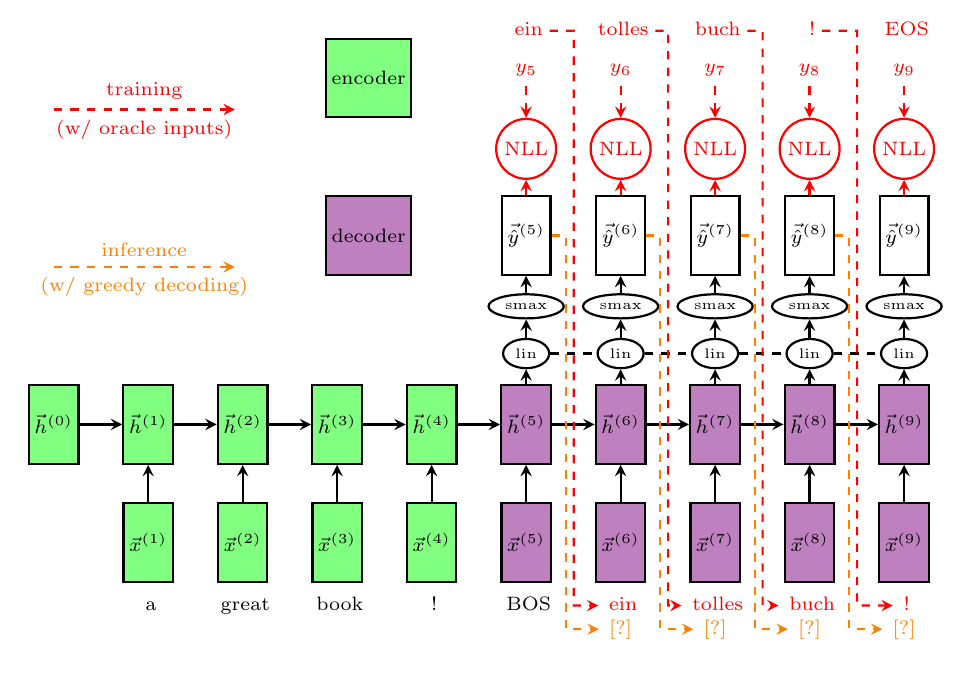
\begin{tikzpicture}[->, thick, >=stealth]
\node [vec, fill=green!50] (h0) at (0,2) {\scriptsize $\vec h^{(0)}$};
\foreach \i/\word/\coll in {1/a/green,2/great/green,3/book/green,4/!/green,5/BOS/violet,6/ein/violet,7/tolles/violet,8/buch/violet,9/!/violet}{
\node [vec, fill=\coll!50] (x\i) at (\i*1.2, .5) {\scriptsize $\vec x^{(\i)}$};
\node [vec, fill=\coll!50] (h\i) at (\i*1.2, 2) {\scriptsize $\vec h^{(\i)}$};
\draw (x\i) -- (h\i);
\pgfmathparse{\i-1};
\draw (h\pgfmathresult) -- (h\i);
}
\foreach \i/\word/\coll in {1/a/green,2/great/green,3/book/green,4/!/green,5/BOS}{
\node (in\i) [text=black, inner sep=-2pt, outer sep=0pt] at (\i*1.2,-.3) {\scriptsize \phantom{A}\word\phantom{g}};
}

\foreach \i/\word/\coll in {6/ein/violet,7/tolles/violet,8/buch/violet,9/!/violet}{
\node (in\i) [text=red, inner sep=-2pt, outer sep=0pt] at (\i*1.2,-.3) {\scriptsize \phantom{A}\word\phantom{g}};
}

\foreach \i/\word in {5/ein,6/tolles,7/buch,8/!,9/EOS}{
\node (smax\i) [draw, ellipse, inner sep=2pt] at (\i*1.2, 3.5) {\tiny smax};
\node (ffn\i) [draw, ellipse, inner sep=2pt] at (\i*1.2, 2.9) {\tiny lin};
\node (pred\i) [vec] at (\i*1.2, 4.4) {\scriptsize $\vec {\hat{y}}^{(\i)}$};
\node (lab\i) [red] at (\i*1.2, 6.5) {\scriptsize ${y}_\i$};
\node (loss\i) [draw, circle, inner sep=2pt, red] at (\i*1.2, 5.5) {\scriptsize NLL};
\node (out\i) [text=red, inner sep=-2pt] at (\i*1.2,7) {\scriptsize \phantom{A}\word\phantom{g}};
\draw  (h\i) -- (ffn\i);
\draw (ffn\i) -- (smax\i);
\draw  (smax\i) -- (pred\i);
\draw (pred\i) [dashed, red] -- (loss\i);
\draw  (lab\i) [dashed, red] -- (loss\i);
}
\draw [dashed, -] (ffn5)--(ffn6)--(ffn7)--(ffn8)--(ffn9);

\draw [dashed, orange] (0, 4) -- node[midway, above, font=\scriptsize] {inference} (2.3,4);
\draw [orange, draw=none] (0, 4) -- node[midway, below, font=\scriptsize] {(w/ greedy decoding)} (2.3,4);
\draw [dashed, red] (0, 6) -- node[midway, above, font=\scriptsize] {training} (2.3,6);
\draw [red, draw=none] (0, 6) -- node[midway, below, font=\scriptsize] {(w/ oracle inputs)} (2.3,6);

\node [vec, fill=green!50] at (4, 6.4) {\scriptsize encoder};
\node [vec, fill=violet!50] at (4, 4.4) {\scriptsize decoder};

\foreach \j/\t in {6/5,7/6,8/7,9/8}{
\pgfmathparse{\j-1};
\node (argmax\j) [text=orange] at (\j*1.2,-.6) {\scriptsize [?]};
\node [xshift=-1.5mm] (pt\j) at ($(ffn\pgfmathresult)!0.5!(ffn\j)$) {};
\node [xshift=-2.5mm] (px\j) at ($(ffn\pgfmathresult)!0.5!(ffn\j)$) {};
\draw [dashed, red] (out\pgfmathresult) -- (pt\j |- out\pgfmathresult) -- (pt\j |- in\j) -- (in\j);
\draw [dashed, orange] (pred\pgfmathresult) -- (px\j |- pred\pgfmathresult) -- (px\j |- argmax\j) -- (argmax\j);
}
\end{tikzpicture}}\end{center}

\vfill

\end{frame}

\begin{vbframe}{Root 2: The Fixed-Size Bottleneck}

\vfill

\begin{itemize}
	\item In an RNN, at a given point in time $j$, the information about all past inputs $x^{(1)} \ldots x^{(j)}$ is ``crammed'' into the state vector $\vec h^{(j)}$ (and $\vec c^{(j)}$ for an LSTM)
	\item So for long sequences, the state becomes a \textbf{bottleneck}
	\item Especially problematic in encoder-decoder models (e.g., for Machine Translation)
	\item Solution: Attention \beamergotobutton{\href{https://arxiv.org/abs/1409.0473}{Bahdanau et al., 2015}} -- an architectural modification of the RNN encoder-decoder that allows the model to ``attend to'' past encoder states
\end{itemize}

\vfill

\end{vbframe}

\begin{vbframe}{Root 2: Bahdanau Attention}

\vfill

\begin{minipage}[c]{.42\textwidth}
\begin{figure}
	\centering
		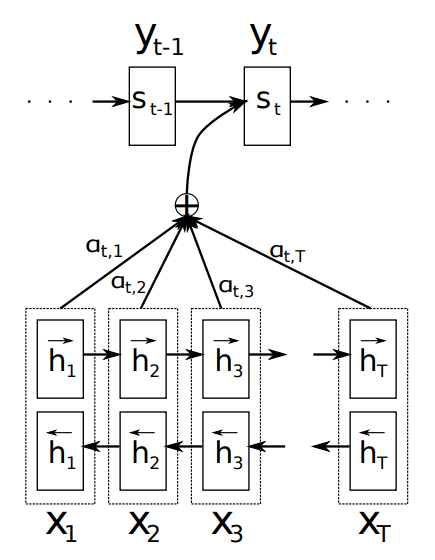
\includegraphics[width = 4.5cm]{figure/bahdanau-attention.png}\\
	\beamergotobutton{\href{https://arxiv.org/abs/1409.0473}{Source: Bahdanau et al., 2015}}
\end{figure}
\end{minipage}
\hfill
\begin{minipage}[c]{.55\textwidth}
\begin{itemize}
	\item The encoder keeps \emph{all} its states $\vec h_1 \ldots \vec h_T$ instead of only the last one.
	\item To produce output $y_t$, the decoder state $s_t$ receives a weighted sum $\sum_j \alpha_{t,j} \vec h_j$ of all encoder states.
	\item The weights $\alpha_{t,j}$ are recomputed at every output step from how relevant $\vec h_j$ is to the current decoder state --- the decoder chooses \emph{where to look} at each step.
\end{itemize}
\end{minipage}

\vfill

\end{vbframe}

\begin{frame}{Root 2: Attention in Practice}
\begin{minipage}[c]{.36\textwidth}
  \centering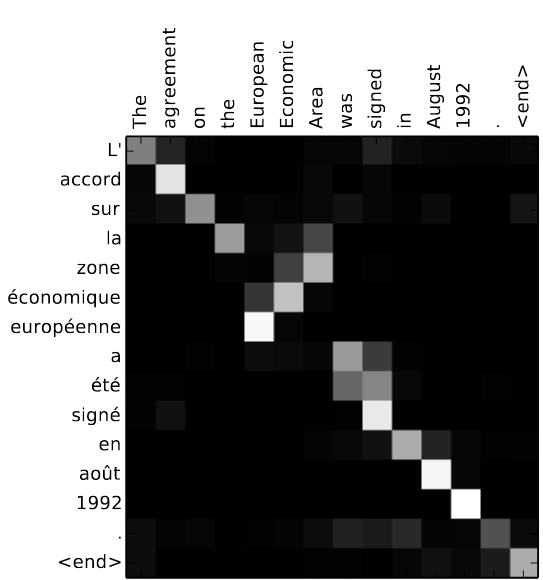
\includegraphics[width=\linewidth,height=2.8cm,keepaspectratio]{figure/bahdanau4.png}
\end{minipage}
\hfill
\begin{minipage}[c]{.6\textwidth}
  \centering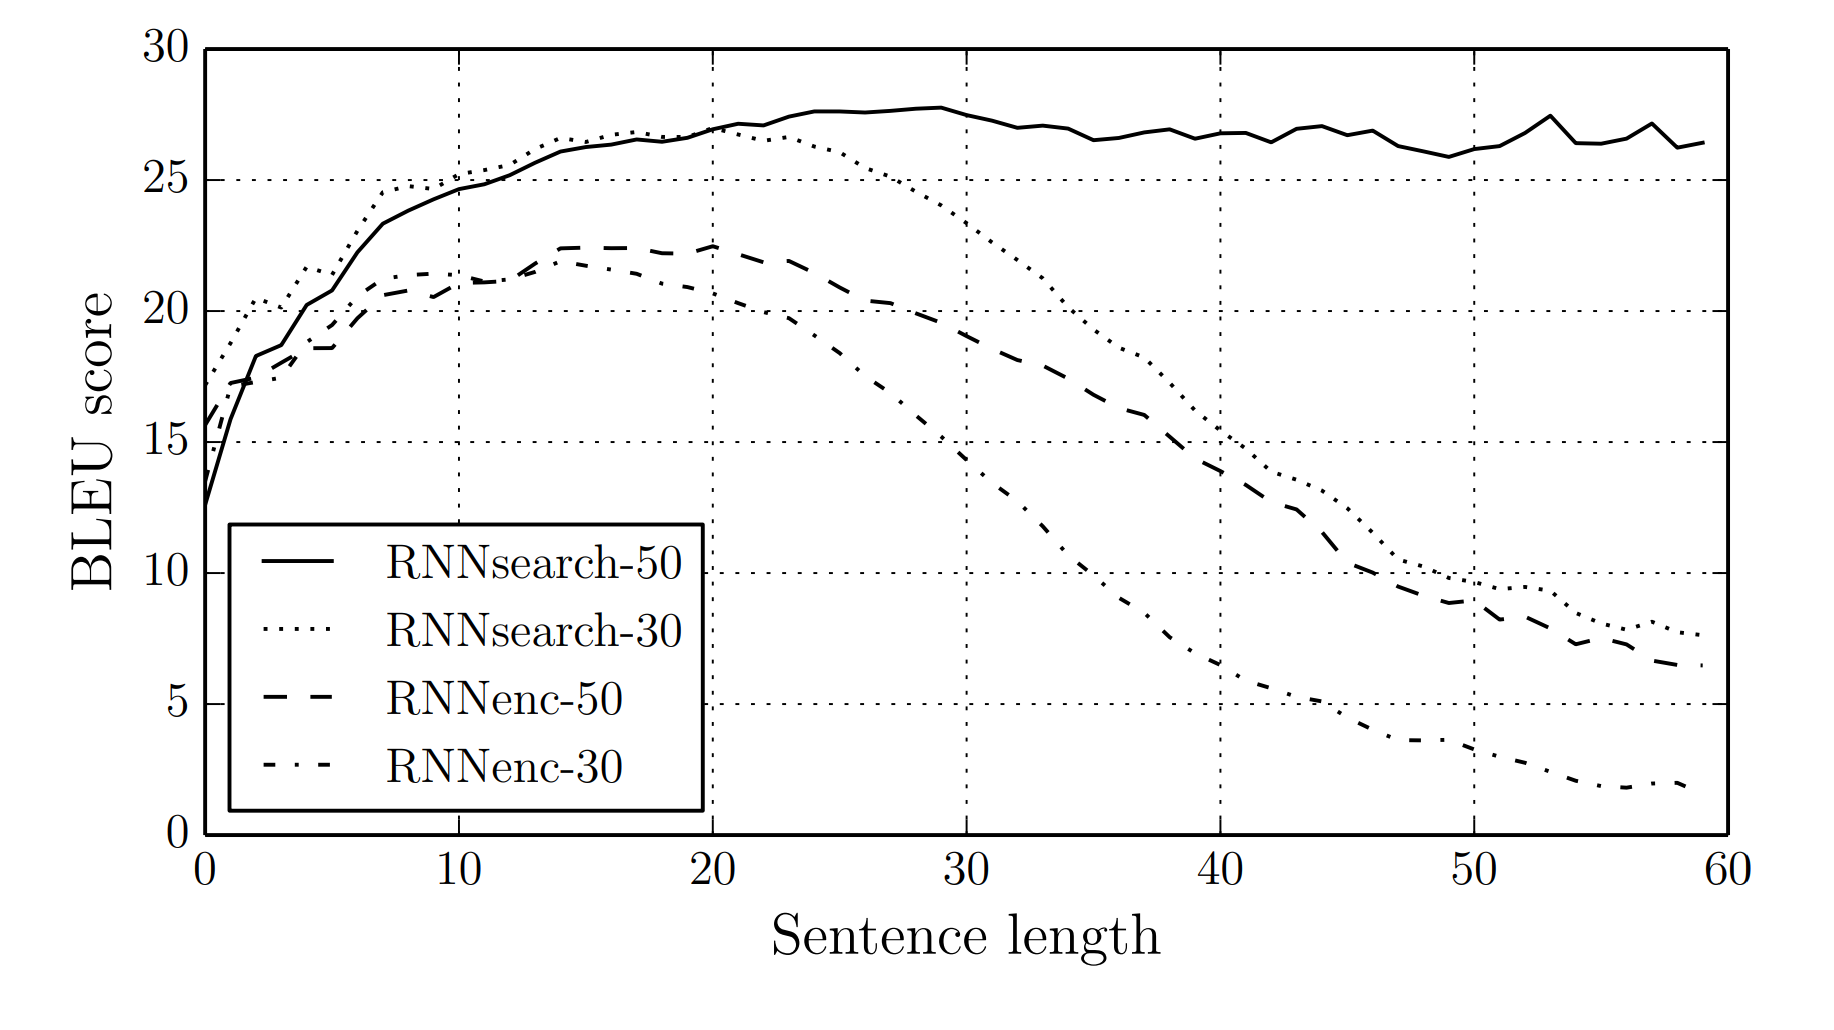
\includegraphics[width=\linewidth,height=2.8cm,keepaspectratio]{figure/bahdanau14.png}
\end{minipage}
\medskip
\small
\begin{itemize}
  \item \textbf{Left}: an attention (alignment) matrix for one translated sentence --- brighter cells mean the decoder attended more strongly to that source word when generating a given target word.
  \item \textbf{Right}: BLEU score (translation quality; higher is better) vs.\ sentence length. \texttt{RNNenc} is the classical fixed-vector encoder-decoder; \texttt{RNNsearch} adds attention. The gap widens sharply on longer sentences --- exactly where a single fixed-size context vector is the tightest bottleneck.
\end{itemize}
{\footnotesize Source: Bahdanau et al.\ (2015).}
\end{frame}

%%%%%%%%%%%%%%%%%%%%%%%%%%%%%%%%%%%%%%%%%%%%%%%%%%%%%%%%%%%%%%%%%%

\section{The Transformer}
%%%%%%%%%%%%%%%%%%%%%%%%%%%%%%%%%%%%%%%%%%%%%%%%%%%%%%%%%%%%%%%%%%

\begin{vbframe}{Machine Translation}

\vfill

\begin{itemize}
	\item Sequence-to-sequence task
	\item Already served as a motivation for introducing the "ordinary" Attention-mechanism \beamergotobutton{\href{https://arxiv.org/abs/1409.0473}{Bahdanau et al., 2015}}
	\item Crucial, that the decoder has access to the whole input sequence \\
				$\to$ This is very well solved by cross-attention
	\item Good contextualization in the encoder improves translation quality
		\begin{itemize}
			\item (Bidirectional) RNNs/LSTMs are only (concatenated) unidirectional architectures
			\item Transformer-Encoder layers are bidirectional by construction
			\item Stacking them on top of each other makes this bidirectional contextualization even "deeper"
		\end{itemize}
\end{itemize}

\vfill

\end{vbframe}

\begin{vbframe}{WMT 2014 EN-to-DE and EN-to-FR}

\vfill

\textbf{Parallel training data:}

\begin{figure}
	\centering
		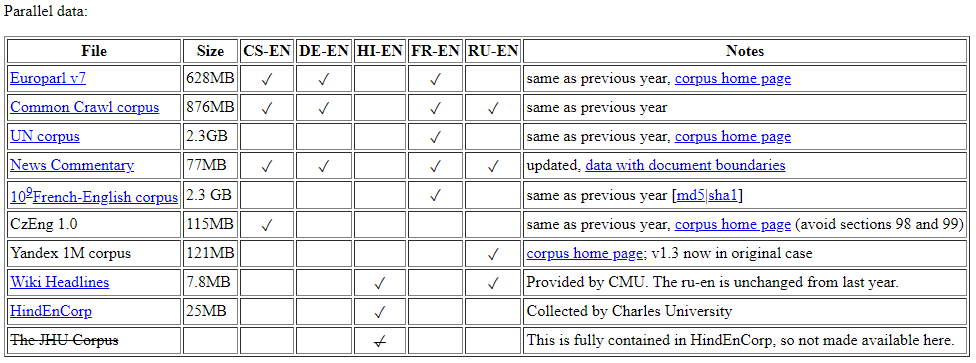
\includegraphics[width=.9\textwidth]{figure/wmt14}
\end{figure}
\vfill

\end{vbframe}

\begin{vbframe}{The BLEU Score}

\vfill

\begin{itemize}
	\item Based on n-gram overlap from candidate and reference sentence
	\item Precision (for each n-gram) calculated as follows:
\end{itemize}

\begin{equation}
            P_{n} = \frac{\sum_{C \in\{\text { Candidates }\}} \sum_{n-g r a m \in C} \text { Count }_{\text {clip }}(n-\text { gram })}{\sum_{C^{\prime} \in\{\text { Candidates }\}}{\sum_{n-g r a m^{\prime} \in C^{\prime}} \text { Count }\left(n-\text { gram }^{\prime}\right)}}  \nonumber
\end{equation}

\begin{itemize}
	\item Finally, the BLEU score can be computed as
\end{itemize}

\begin{equation}
            \texttt{BLEU} = BP \cdot \exp\left(\sum_{n=1}^{N} w_n \cdot \log(P_n)\right), \nonumber
\end{equation}

\begin{itemize}
	\item where $BP$ is a "brevity penalty" to penalize short generations, $N$ is the number of n-grams \& $w_n$ the weight for each $P_n$ (usually $\frac{1}{N}$)
\end{itemize}

\vfill

\end{vbframe}

\begin{frame}{Transformer for MT}
\small

\vfill

The Transformer ..

\begin{itemize}
	\item .. outperforms the previous SOTA models
	\item .. at a lower number of required training FLOPs
\end{itemize}

\vspace{.3cm}

\begin{figure}
	\centering
		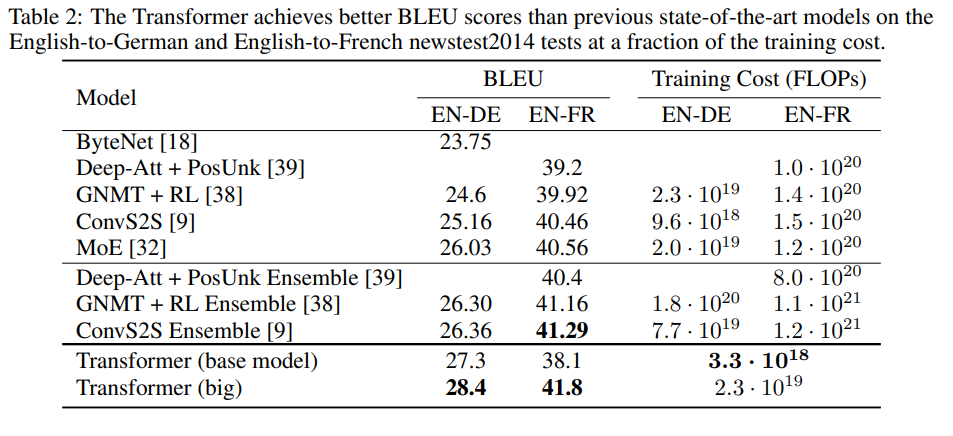
\includegraphics[width=.8\textwidth]{figure/trafo-wmt}\\
	\beamergotobutton{\href{https://arxiv.org/abs/1706.03762}{Source: Vaswani et al., 2017}}
\end{figure}

\vfill

\end{frame}

\begin{frame}{The Transformer architecture}

\begin{center}
\resizebox{!}{.74\textheight}{\begin{tikzpicture}[->, >=stealth, thick, font=\scriptsize]
\node (transformer) at (0,0) {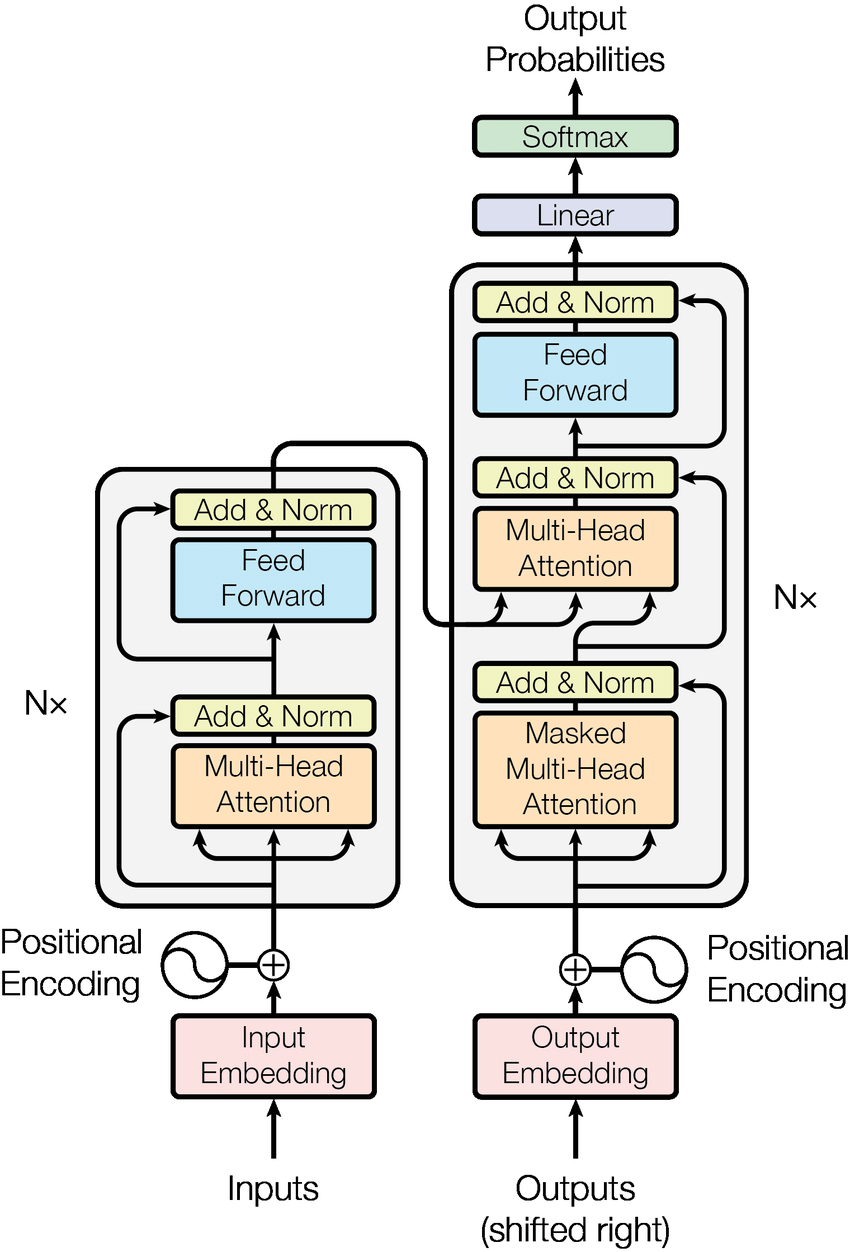
\includegraphics[width=.4\textwidth]{figure/transformer.png}};
\node (enc) [left=2mm of transformer, rotate=90] {encoder};
\node (dec) [right=2mm of transformer, rotate=270] {decoder};
\node (x) [above left=1cm of transformer.south west] {$X$ (source)};
\node (y) [above right=1cm of transformer.south east] {$Y$ (target)};
\draw (x) -- ([yshift=5mm, xshift=1cm] transformer.south west);
\draw (y) -- ([yshift=5mm, xshift=-1cm] transformer.south east);
\node (nll) [draw, circle] at ([yshift=-5mm] transformer.north east) {NLL};
\draw [bend right=55] (y.north east) to (nll);
\draw ([xshift=-1cm, yshift=-5mm] transformer.north east) to (nll);
\node at (-3, 2) [align=left] {(For simpler problems (e.g., \\ classification, tagging), \\ you would simply use \\ the encoder.)};
\end{tikzpicture}}\\
	\beamergotobutton{\href{https://arxiv.org/abs/1706.03762}{Source: Vaswani et al., 2017}}
\end{center}

\end{frame}

%%%%%%%%%%%%%%%%%%%%%%%%%%%%%%%%%%%%%%%%%%%%%%%%%%%%%%%%%%%%%%%%%%

\section{Tokenization}
%%%%%%%%%%%%%%%%%%%%%%%%%%%%%%%%%%%%%%%%%%%%%%%%%%%%%%%%%%%%%%%%%%

\begin{vbframe}{Process of Text Tokenization}
\begin{itemize}
  \item The Transformer above consumes a sequence of ``tokens''. Tokenization is the preprocessing step that produces them: breaking raw text into smaller discrete units (letters, words, sub-words, ...) and encoding each unique unit with an integer ID.
  \item Performed once over an entire corpus, this yields a fixed \textbf{vocabulary} of unique tokens --- the set of IDs the model's embedding lookup table must cover.
  \item A mandatory preprocessing step for essentially every NLP task, and the direct source of the token sequences fed into every Transformer frame in this session.
\end{itemize}
\end{vbframe}

\begin{vbframe}{Why Tokenize?}
\begin{itemize}
  \item Text must be turned into numbers before any neural network can process it; the question is only which granularity to encode.
  \item Whole documents are too large and unstructured to model directly --- meaning is built bottom-up from smaller units.
  \item Tokenization also normalizes incidental formatting (extra whitespace, casing, punctuation spacing) that carries no meaning.
\end{itemize}
\end{vbframe}

\begin{vbframe}{Tokenization in Action}
\begin{figure}
  \centering
  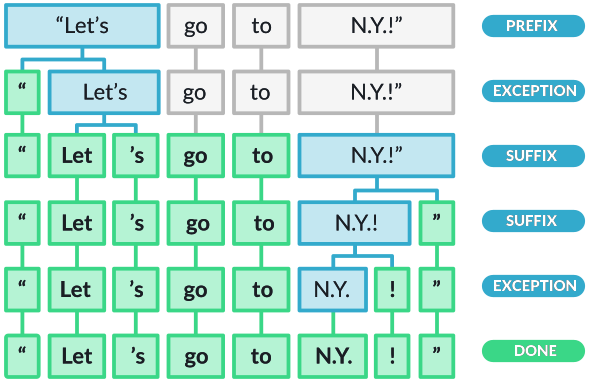
\includegraphics[width=9cm]{figure/spacy_tok.png}\\
  \footnotesize{Source:} \href{https://spacy.io/usage/linguistic-features}{\footnotesize spaCy}
\end{figure}
\end{vbframe}

\begin{vbframe}{Tokenization Types}
\begin{itemize}
  \item \textbf{Word tokenization}: split on whitespace/punctuation --- most common, but a fixed vocabulary can't cover every word that will ever appear.
  \item \textbf{Subword tokenization}: split words into smaller meaningful (or at least frequent) units --- the standard choice for modern Transformers.
  \item \textbf{Character tokenization}: split into individual characters --- tiny vocabulary, no out-of-vocabulary problem, but much longer sequences.
  \item (Paragraph, sentence, and whitespace tokenization also exist, as coarser or purely mechanical splits; rarely the final step for a Transformer's input.)
\end{itemize}
\end{vbframe}

\begin{vbframe}{Word, Subword, and Character Tokenization}
\textbf{Word tokenization} --- whitespace and punctuation mark boundaries:
\begin{quote}
\small\it "What is the tallest building?" $\to$ \{What, is, the, tallest, building, ?\}
\end{quote}
Simple and interpretable, but the vocabulary must contain every word form the model will ever see, or it falls back to an ``unknown token'' and loses information.

\framebreak

\textbf{Subword tokenization} --- split words into smaller, more frequent units (roots, prefixes, suffixes):
\begin{quote}
\small\it "What is the tallest building?" $\to$ \{What, is, the, tall, est, build, ing, ?\}
\end{quote}
Keeps the vocabulary small while still generalizing to unseen word forms --- important for morphologically rich languages, and the choice essentially every modern Transformer makes.

\framebreak

\textbf{Character tokenization} --- split into individual characters:
\begin{quote}
\small\it "What...?" $\to$ \{W, h, a, t, ..., ?\}
\end{quote}
No out-of-vocabulary words are possible at all (any string is just a sequence of known characters), at the cost of much longer sequences --- and, as we will see, self-attention's cost scales quadratically with sequence length.
\end{vbframe}

%%%%%%%%%%%%%%%%%%%%%%%%%%%%%%%%%%%%%%%%%%%%%%%%%%%%%%%%%%%%%%%%%%

\section{Attention, Formalized}
%%%%%%%%%%%%%%%%%%%%%%%%%%%%%%%%%%%%%%%%%%%%%%%%%%%%%%%%%%%%%%%%%%

\begin{vbframe}{Attention: The Basic Recipe (1)}

\vfill

\begin{itemize}
	\item \textbf{Ingredients:}
	\item[]
	\item One query vector: $\mathbf{q} \in \mathbb{R}^{d_q}$
	\item J key vectors: $\mathbf{K} \in \mathbb{R}^{J \times d_k}; (\vec k_1 \ldots \vec k_J)$
	\item J value vectors: $\mathbf{V} \in \mathbb{R}^{J \times d_v}; (\vec v_1 \ldots \vec v_J)$
	\item Scoring function $a : \mathbb{R}^{d_q} \times \mathbb{R}^{d_k} \rightarrow \mathbb{R}$
		\begin{itemize}
			\item Maps a query-key pair to a scalar (``score'')
			\item $a$ may be parametrized by parameters $\theta_a$
		\end{itemize}
\end{itemize}

\vfill

\end{vbframe}

\begin{vbframe}{Attention: The Basic Recipe (2)}

\vfill

\begin{itemize}
	\item \textbf{Step 1}: Apply $a$ to $\vec q$ and all keys $\vec k_j$ to get scores (one per key): 
	$$\vec e = \begin{bmatrix} e_1 \\ \vdots \\ e_J \end{bmatrix} =  \begin{bmatrix} a(\vec q, \vec k_1; \theta_a) \\ \vdots \\ a(\vec q, \vec k_J; \theta_a) \end{bmatrix}$$
	\item \textbf{Step 2}: Turn $\mathbf{e}$ into a probability distribution with the softmax function
	$$\alpha_j = \frac{\mathrm{exp}(e_j)}{\sum_{j'=1}^J \mathrm{exp}(e_{j'})}$$
		\begin{itemize}
			\item Note that $\sum_j \alpha_j = 1$
		\end{itemize}
\end{itemize}

\vfill

\end{vbframe}

\begin{vbframe}{Attention: The Basic Recipe (3)}

\vfill

\begin{itemize}
	\item \textbf{Step 3}: $\alpha$-weighted sum over $\vec {V}$ yields one $d_v$-dimensional output vector:
	$$\vec {o} = \sum_{j=1}^J \alpha_j \vec {v}_j$$
		\begin{itemize}
			\item Intuition: $\alpha_j$ is how much ``attention'' the model pays to $\vec v_j$ when computing $\vec o$.
		\end{itemize}
	\item In a neural network, $\vec q$, $\vec k_j$ and $\vec v_j$ are functions of the input and of trainable parameters
	\item So the \textit{model} learns which keys are relevant for which queries, based on the training data and loss function
\end{itemize}

\vfill

\end{vbframe}

\begin{vbframe}{Attention in the Transformer}

\vfill

\begin{itemize}
\item We can use attention on many different ``things'', including:
\begin{itemize}
\item The pixels of images
\item The nodes of knowledge graphs
\item The words of a vocabulary
\end{itemize}
\item Here, we focus on scenarios where the query, key and value vectors represent tokens (e.g., words, characters, etc.) in sequences (e.g., sentences, paragraphs, etc.).
\end{itemize}

\vfill

\end{vbframe}

\begin{vbframe}{Attention in the Transformer}

\vfill

\textbf{Cross-Attention:}
\begin{itemize}
\item Let $X = (x_1 \ldots x_{J_x}), Y = (y_1 \ldots y_{J_y})$ be two sequences (e.g., source and target in a sequence-to-sequence problem)
\item The query vectors represent tokens in $Y$ and the key/value vectors represent tokens in $X$ (``$Y$ attends to $X$'')
\end{itemize}

\medskip\medskip

\textbf{Self-Attention:}
\begin{itemize}
\item There is only one sequence $X = (x_1 \ldots x_J)$
\item The query, key and value vectors represent tokens in $X$ (``$X$ attends to itself'')
\end{itemize}

\vfill

\end{vbframe}

\begin{vbframe}{Cross-Attention (1)}

\vfill

\begin{itemize}
	\item We start by describing cross-attention, self-attention can easily be derived by assuming $\vec X = \vec Y$.
	\item Let $\vec X \in \mathbb{R}^{J_x \times d_x}, \vec Y \in \mathbb{R}^{J_y \times d_y}$ be representations of $X, Y$ (e.g., stacked word embeddings, or the outputs of a previous layer)
	\item Let $\theta = \{\vec W^{(q)} \in \mathbb{R}^{d_y \times d_q}, \vec W^{(k)} \in \mathbb{R}^{d_x \times d_k}, \vec W^{(v)} \in \mathbb{R}^{d_x \times d_v}\}$\\ be trainable weight matrices
	\item We transform $\vec Y$ into a matrix of query vectors:
	$$ \vec Q = \vec Y \vec W^{(q)} $$
	\item We transform $\vec X$ into matrices of key and value vectors:
	$$ \vec K = \vec X \vec W^{(k)} ; \qquad \vec V =  \vec X \vec W^{(v)}$$
\end{itemize}

\vfill

\end{vbframe}

\begin{vbframe}{Cross-Attention (2)}

\vfill

\begin{itemize}
	\item To calculate the $e$ scores, Vaswani et al. use a parameter-less scaled dot product instead of Bahdanau's complicated FFN\medskip\medskip
	\item Step 1 of the basic recipe: \textit{Scores}
	$$ e_{j,j'} = a(\vec q_j, \vec k_{j'}) = \frac{\vec q_j^T \vec k_{j'}}{\sqrt{d_k}} $$
	\item Note: This requires that $d_q = d_k$
\end{itemize}

\vfill

\end{vbframe}

\begin{vbframe}{Cross-Attention (3)}

\vfill

\begin{itemize}
	\item Attention weights and outputs are defined like before\medskip\medskip
	\item Step 2 of the basic recipe: \textit{Weights}
	$$ \alpha_{j,j'} = \frac{\mathrm{exp}(e_{j,j'})}{\sum_{j'' = 1}^{J_x} \mathrm{exp}(e_{j,j''})}$$
	\item Step 3 of the basic recipe: \textit{Outputs}
	$$ \vec o_j = \sum_{j'=1}^{J_x} \alpha_{j,j'} \vec v_{j'}$$
\end{itemize}

\vfill

\end{vbframe}

\begin{frame}{Cross-Attention (4)}

\vskip-2mm
\resizebox{!}{.8\textheight}{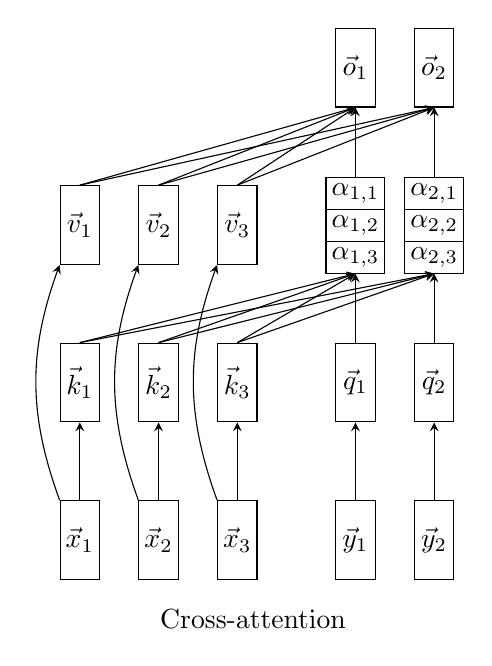
\begin{tikzpicture}[->, >=stealth]
\foreach \x in {1,2,3}{
\node (x\x) [vec] at (\x, -.5) {$\vec x_\x$};
\node (k\x) [vec] at (\x, 1.5) {$\vec k_\x$};
\node (v\x) [vec] at (\x, 3.5) {$\vec v_\x$};
}
\foreach \y in {1,2}{
\node (y\y) [vec] at (\y+3.5, -.5) {$\vec y_\y$};
\node (q\y) [vec] at (\y+3.5,1.5) {$\vec q_\y$};
\node (o\y) [vec] at (\y+3.5,5.5) {$\vec o_\y$};
\node (alpha\y) [vec, rectangle split, rectangle split parts=3] at (\y+3.5,3.5) {\nodepart{one} $\alpha_{\y,1}$ \nodepart{two} $\alpha_{\y,2}$ \nodepart{three} $\alpha_{\y,3}$};
}

\foreach \y in {1,2}{
\draw (alpha\y.north) -- (o\y.south);
\draw (q\y.north) -- (alpha\y.south);
\draw (y\y.north) -- (q\y.south);
\foreach \x in {1,2,3}{
\draw (v\x.north) -- (o\y.south);
\draw (k\x.north) -- (alpha\y.south);
}}
\foreach \x in {1,2,3}{
\draw (x\x.north) -- (k\x.south);
\draw [bend left=20] (x\x.north west) to (v\x.south west);
}
\node at (3.2, -1.5) {Cross-attention};
\end{tikzpicture}}

\end{frame}

\begin{frame}{Self-Attention}

\vskip-2mm
\hfill
\resizebox{!}{.8\textheight}{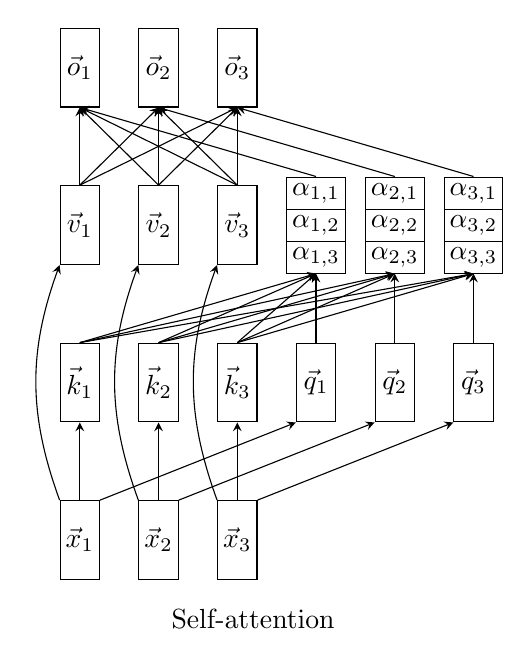
\begin{tikzpicture}[->, >=stealth]
\foreach \x in {1,2,3}{
\node (x\x) [vec] at (\x, -.5) {$\vec x_\x$};
\node (k\x) [vec] at (\x, 1.5) {$\vec k_\x$};
\node (v\x) [vec] at (\x, 3.5) {$\vec v_\x$};
}
\foreach \y in {1,2,3}{
\node (q\y) [vec] at (\y+3,1.5) {$\vec q_\y$};
\node (o\y) [vec] at (\y,5.5) {$\vec o_\y$};
\node (alpha\y) [vec, rectangle split, rectangle split parts=3] at (\y+3,3.5) {\nodepart{one} $\alpha_{\y,1}$ \nodepart{two} $\alpha_{\y,2}$ \nodepart{three} $\alpha_{\y,3}$};
}

\foreach \y in {1,2,3}{
\draw (alpha\y.north) -- (o\y.south);
\draw (q\y.north) -- (alpha\y.south);
\draw (x\y.north east) -- (q\y.south west);
\foreach \x in {1,2,3}{
\draw (v\x.north) -- (o\y.south);
\draw (k\x.north) -- (alpha\y.south);
}}
\foreach \x in {1,2,3}{
\draw (x\x.north) -- (k\x.south);
\draw [bend left=20] (x\x.north west) to (v\x.south west);
}
\node at (3.2, -1.5) {Self-attention};
\end{tikzpicture}}

\end{frame}

\begin{vbframe}{Self-Attention Formalized}

\vfill

\begin{itemize}
\item Let $\vec X \in \mathbb{R}^{J_x \times d_x}$ be a representation of $X$ (e.g., stacked word embeddings, or the outputs of a previous layer)
\item Let $\theta = \{\vec W^{(q)} \in \mathbb{R}^{d_x \times d_q}, \vec W^{(k)} \in \mathbb{R}^{d_x \times d_k}, \vec W^{(v)} \in \mathbb{R}^{d_x \times d_v}\}$\\ be trainable weight matrices
\item We transform $\vec X$ into a matrix of query vectors:
$$ \vec Q = \vec X \vec W^{(q)} $$
\item And we transform $\vec X$ into matrices of key and value vectors:
$$ \vec K = \vec X \vec W^{(k)} ; \qquad \vec V =  \vec X \vec W^{(v)}$$
\item Execute Steps 1 -- 3 of the basic recipe
\end{itemize}

\vfill

\end{vbframe}

\begin{frame}{A General Property: Permutation Invariance/Equivariance}
\footnotesize
\begin{itemize}
  \item For a permutation $\sigma$ of sequence positions, standard attention is:
  \begin{itemize}
    \item \textbf{invariant} to a permutation of the keys and values: $Y(\vec Q, \sigma(\vec K), \sigma(\vec V)) = Y(\vec Q, \vec K, \vec V)$,
    \item \textbf{equivariant} to a permutation of the queries: $Y(\sigma(\vec Q), \vec K, \vec V) = \sigma(Y(\vec Q, \vec K, \vec V))$.
  \end{itemize}
  \item Consequently, self-attention (where $\vec Q, \vec K, \vec V$ all come from the same sequence) is equivariant to a permutation of its input: reorder the tokens and the outputs simply reorder the same way --- \textbf{the values themselves don't change}.
  \item So self-attention alone cannot tell \textit{where} in the sequence a token is, only \textit{what} the other tokens are. The next frames show what goes wrong, and how position embeddings fix it.
\end{itemize}
{\footnotesize Framing after Fleuret, \textit{Deep Learning} (UNIGE) \S13.2, CC BY-NC-SA 4.0.}
\end{frame}

\begin{vbframe}{Can Self-Attention Model Word Order?}

\vfill

\begin{itemize}
	\item Hypothetical model:
			\begin{itemize}
				\item simple word embedding lookup layer
				\item self-attention layer
			\end{itemize}
	\item Let $\blu{X^{(1)}}$, $\org{X^{(2)}}$ be two sentences of the same length $J$, which contain the same words, but in a different order
	\item Example: \blu{``john loves mary''} vs. \org{``mary loves john''}
\end{itemize}
\begin{center}
	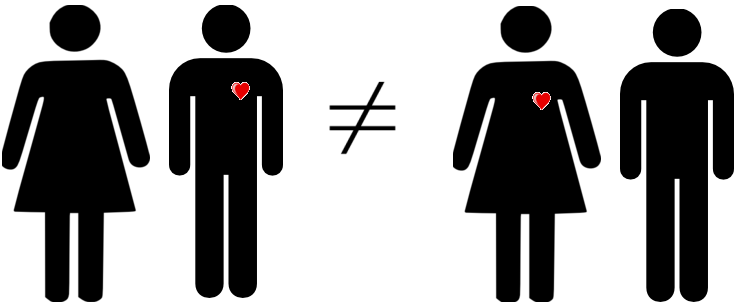
\includegraphics[width=.6\textwidth]{figure/mary_loves_john}
\end{center}

\vfill

\end{vbframe}

\begin{frame}{Can Self-Attention Model Word Order?}
\footnotesize

\vfill

\begin{itemize}
\item By the permutation equivariance above: reordering the input tokens only reorders the outputs, it never changes them.
\item In other words: The representation of \blu{mary} is identical to that of \org{mary}, and the representation of \blu{john} is identical to that of \org{john}
\item \ques Can the other layers in the Transformer architecture (feed-forward net, layer normalization) help with the problem?
\begin{itemize}
\item No, because they apply the same function to all positions.
\end{itemize}
\item \ques Would it help to apply more self-attention layers?
\begin{itemize}
\item No. Since the representations of identical words are still identical in $\vec O$, the next self-attention layer will have the same problem.
\end{itemize}
\item Luckily, we just need to ensure that input embeddings of identical words at different positions are not identical.
\end{itemize}

\vfill

\end{frame}

\begin{vbframe}{Position Embeddings}

\vfill

\begin{itemize}
\item Add to every input word embedding a position embedding $\vec {p} \in \mathbb{R}^d$:
\item Input embedding of word ``mary'' in position $j$: $\vec {x}_j = \vec {w}_{\mathcal{I}(\text{mary})} + \mathbf{p}_j$
$$\vec {w}_{\mathcal{I}(\text{mary})} + \vec {p}_j \neq \vec{w}_{\mathcal{I}(\text{mary})} + \vec {p}_{j'} \text{ if } j \neq j'$$
\item Option 1 \beamergotobutton{\href{https://arxiv.org/abs/1706.03762}{Source: Vaswani et al., 2017}}\\
(Deterministic) Sinusoidal position embeddings:
$$p_{j,i} = \begin{cases} \mathrm{sin}\big(\frac{j}{10000^\frac{i}{d}}\big)  & \text{ if } i \text{ is even} \\ \mathrm{cos}\big(\frac{j}{10000^\frac{i-1}{d}}\big) & \text{ if } i \text{ is odd}  \end{cases}$$
\item Option 2 \beamergotobutton{\href{https://aclanthology.org/N19-1423.pdf}{Source: Devlin et al., 2019}}\\
Trainable position embeddings: $\vec {P} \in \mathbb{R}^{J^\mathrm{max} \times d}$\\
(Disadvantage: Cannot deal with sentences longer than $J^\mathrm{max}$)
\end{itemize}

\vfill

\end{vbframe}

\begin{vbframe}{Parallelized Attention}

\vfill

\begin{itemize}
\item We want to apply our attention recipe to every query vector $\vec q_j$
\item We could simply loop over all time steps $1 \leq j \leq J_x$ (or $J_y$) and calculate each $\vec o_j$ independently.
\item Then stack all $\vec o_j$ into an output matrix $\vec O \in \mathbb{R}^{J_x \times d_v}$ (or $\mathbb{R}^{J_y \times d_v}$)
\item But a loop does not use the GPU's capacity for parallelization,\\ so it might be unnecessarily slow
\end{itemize}

\vfill

\end{vbframe}

\begin{vbframe}{Parallelized Self-Attention}

\vfill

\begin{itemize}
\item Do some inputs (e.g., $\vec q_j$) depend on previous outputs (e.g., $\vec o_{j-1}$)? If not, we can parallelize the loop into a single function:
$$\vec O = \mathcal{F}^\mathrm{attn}(\vec X, \vec X; \theta)$$
\item Attention in Transformers is usually parallelizable, unless we are doing autoregressive inference (more on that later).
\end{itemize}

\vfill

\end{vbframe}

\begin{vbframe}{Parallelized Self-Attention}

\vfill

\begin{itemize}
\item By the way: The Bahdanau model is not parallelizable in this way, because $s_i$ (a.k.a. the query of the $i+1$'st step) depends on $c_i$ (a.k.a. the attention output of the $i$'th step):
\begin{center}
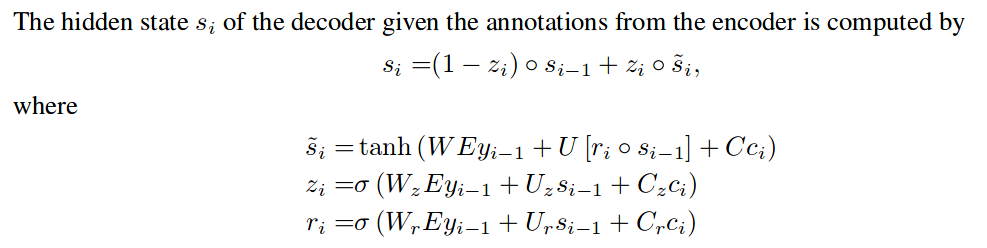
\includegraphics[width=.9\textwidth]{figure/bahdanau3}
\end{center}
\end{itemize}

\vfill

\end{vbframe}

\begin{vbframe}{Parallelized Self-Attention}

\vfill

\begin{itemize}
\item \textbf{Step 1}: The parallel application of the scaled dot product to all query-key pairs can be written as:
$$\vec {E} = \frac{ \vec {Q} \vec {K}^T}{\sqrt{d_k}}; \quad \vec E \in \mathbb{R}^{J_x \times J_x}$$
$$ \frac{1}{\sqrt{d_k}}
\begin{bmatrix}
- & \vec q_1  & -  \\
& \vdots & \\
-  & \vec q_{J_x}  &  -  \\
\end{bmatrix}
\begin{bmatrix}
\lvert &  & \lvert  \\
\vec k_1 & \ldots & \vec k_{J_x} \\
\lvert &  & \lvert  \\
\end{bmatrix}
=
\begin{matrix} \downarrow \\ queries \\ \downarrow \\ \end{matrix} \overset{\rightarrow keys \rightarrow}{
\begin{bmatrix}
e_{1,1} & \ldots & e_{1,J_x} \\
\vdots & \ddots & \vdots \\
e_{J_x,1} & \ldots & e_{J_x,J_x} \\
\end{bmatrix}}$$
\end{itemize}

\vfill

\end{vbframe}

\begin{vbframe}{Parallelized Scaled Dot Product Self-Attention}

\vfill

\begin{itemize}
\item \textbf{Step 2}: Softmax with normalization over the second axis (key axis):
$$\alpha_{j,j'} = \frac{\mathrm{exp}(e_{j,j'})}{\sum_{j''=1}^{J_x} \mathrm{exp}(e_{j,j''})}$$
\item Let's call this new normalized matrix $\vec A \in (0,1)^{J_x \times J_x}$
\item The rows of $\vec A$, denoted $\vec \alpha_j$, are probability distributions\\ (one $\vec \alpha_j$ per $\vec q_j$)
\end{itemize}

\vfill

\end{vbframe}

\begin{vbframe}{Parallelized Scaled Dot Product Self-Attention}

\vfill

\begin{itemize}
\item \textbf{Step 3}: Weighted sum
$$\vec {O} = \vec {A} \vec {V}; \vec O \in \mathbb{R}^{J_x \times d_v}$$

$$
\begin{bmatrix}
- & \boldsymbol \alpha_1  & -  \\
& \vdots & \\
-  & \boldsymbol \alpha_{J_x}  &  -  \\
\end{bmatrix}
\begin{bmatrix}
\lvert &  & \lvert  \\
\vec {v}_{:,1} & \ldots & \vec {v}_{:,d_v} \\
\lvert &  & \lvert  \\
\end{bmatrix}
=
\begin{matrix} \downarrow \\ queries \\ \downarrow \end{matrix}
	\overset{\rightarrow d_v \text{(value dims)} \rightarrow}{
\begin{bmatrix}
o_{1,1} & \ldots & o_{1,d_v} \\
\vdots & \ddots & \vdots \\
o_{J_x,1} & \ldots & o_{J_x,d_v} \\
\end{bmatrix}}
$$
\end{itemize}

\vfill

\end{vbframe}

\begin{vbframe}{... as a One-Liner}

\vfill

\large
$$ \vec O = \mathcal{F}^\mathrm{attn}(\vec X, \vec X; \theta) = \mathrm{softmax}\Big(\frac{(\vec X\vec W^{(q)} ) (\vec X\vec W^{(k)} )^T}{\sqrt{d_k}}\Big)(\vec X\vec W^{(v)} ) $$
\begin{itemize}
\item GPUs like matrix multiplications\\$\rightarrow$ usually a lot faster than RNN!
\item But: The memory requirements of $\vec E$ and $\vec A$ are $\mathcal{O}(J_x^2)$
\item Sequence lengths are an important issue.
\end{itemize}

\vfill

\end{vbframe}

\begin{frame}{Add-On: Changes for Cross-Attention}
\small

\vfill

\begin{itemize}
	  \item \textbf{Step 1}: Scaled dot-product $$\vec {E} = \frac{ \vec {Q} \vec {K}^T}{\sqrt{d_k}}; \quad \vec E \in \mathbb{R}^{J_y \times J_x}$$
	  \item \textbf{Step 2}: Softmax $$\alpha_{j,j'} = \frac{\mathrm{exp}(e_{j,j'})}{\sum_{j''=1}^{J_x} \mathrm{exp}(e_{j,j''})}$$
		\item \textbf{Step 3}: Output $$\vec {O} = \vec {A} \vec {V}; \vec O \in \mathbb{R}^{J_y \times d_v}$$
		\item As one-liner: $$ \vec O = \mathcal{F}^\mathrm{attn}(\vec X, \vec Y; \theta) = \mathrm{softmax}\Big(\frac{(\vec Y\vec W^{(q)} ) (\vec X\vec W^{(k)} )^T}{\sqrt{d_k}}\Big)(\vec X\vec W^{(v)} ) $$
\end{itemize}

\vfill

\end{frame}

\begin{vbframe}{Multi-Layer Attention}

\vfill

\begin{itemize}
\item Sequential application of several attention layers, with separate parameters $\{\theta^{(1)} \ldots \theta^{(N)}\}$
\item In Transformer: sequential application of Transformer blocks
\item There are some additional position-wise layers inside the Transformer block, i.e., $\vec O^{(n)}$ undergoes some additional transformations before becoming the input to the next Transformer block $n+1$
\end{itemize}

\vfill

\end{vbframe}

\begin{vbframe}{Multi-Head Attention}

\vfill

\begin{itemize}
\item Application of several attention layers (``heads'') in parallel
\item $M$ sets of parameters $\{\theta^{(1)}, \ldots, \theta^{(M)}\}$, with $\theta^{(m)} = \{\vec {W}^{(m,q)}, \vec {W}^{(m,k)}, \vec {W}^{(m,v)}\}$
\item For every head, compute in parallel:
$$ \vec O^{(m)} = \mathcal{F}^\mathrm{attn}(\vec X, \vec Y; \theta^{(m)}) $$
\item Choice of dimensionality: $d_k = d_v = d_{x}/M$
\item Concatenate all $\vec {O}^{(m)}$ along their last axis; then down-project the concatenation with an additional parameter matrix $\vec W^{(o)} \in \mathbb{R}^{Md_v \times d_x}$:
$$ \vec O = [\vec O^{(1)}; \ldots;  \vec O^{(M)}] \vec W^{(o)}$$
\end{itemize}

\vfill

\end{vbframe}

\begin{frame}{Multi-Head Attention}
\small

\vfill

\begin{itemize}
\item Conceptually, multi-head attention is to single-head attention like a filter bank is to a single filter (CNNs)
\item Division of labor: different heads model different kinds of inter-word relationships
\end{itemize}

	\begin{figure}
		\centering
		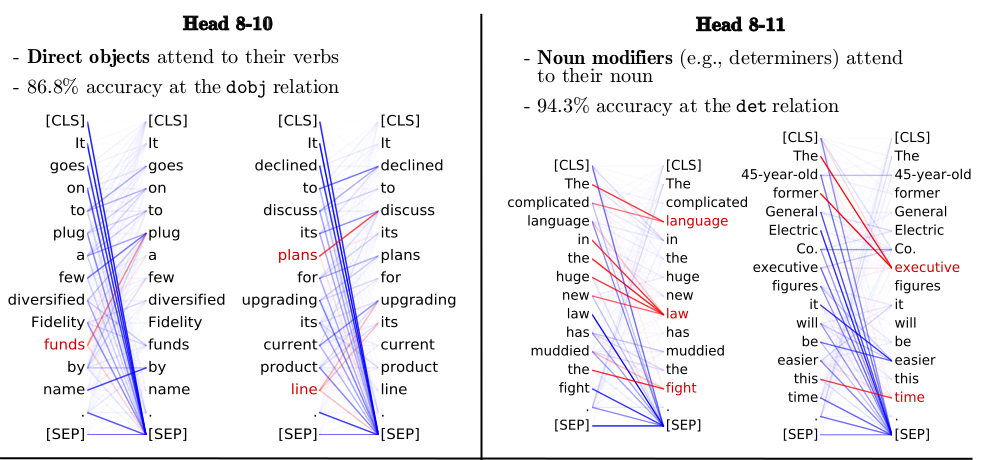
\includegraphics[width = 9cm]{figure/heads.png}\\
		\beamergotobutton{\href{https://aclanthology.org/W19-4828/}{Source: Clark et al., 2019}}
	\end{figure}

\vfill

\end{frame}

%%%%%%%%%%%%%%%%%%%%%%%%%%%%%%%%%%%%%%%%%%%%%%%%%%%%%%%%%%%%%%%%%%

\section{The Transformer Block}
%%%%%%%%%%%%%%%%%%%%%%%%%%%%%%%%%%%%%%%%%%%%%%%%%%%%%%%%%%%%%%%%%%

\begin{vbframe}{Residual Connections}

\vfill

\begin{itemize}
\item Let $\mathcal{F}$ be a function with parameters $\theta$
\item $\mathcal{F}$ with a residual connection:
$$\mathcal{F}'(\vec X; \theta) = \mathcal{F}(\vec X; \theta) + \vec X$$
\begin{center}
\vfill
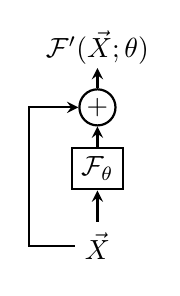
\begin{tikzpicture}[->, >=stealth, thick]
\node (layer) at (0,0) [draw, rectangle, minimum size = 5mm] {$\mathcal{F}_\theta$};
\node (h) [above=1cm of layer, inner sep=1pt] {$\mathcal{F}'(\vec X; \theta)$};
\node (plus) [draw, circle, inner sep=1pt] at ($(layer.north)!0.5!(h.south)$) {$+$};
\node (left) [left=5mm of layer, inner sep=0pt] {};
\node (x) [below=4mm of layer] {$\vec X$};
\draw (x) -- (left |- x) -- (left |- plus) -- (plus);
\draw (x) -- (layer);
\draw (layer) -- (plus);
\draw (plus) -- (h);
\end{tikzpicture}
\end{center}
\item Benefits: Information retention (we add to $\vec X$ but don't replace it)
\end{itemize}

\vfill

\end{vbframe}

\begin{frame}{Layer Normalization}
\footnotesize

\vfill

\begin{itemize}
\item Let $\theta = \{\vec \gamma \in \mathbb{R}^d, \vec \beta \in \mathbb{R}^d\}$ be trainable parameters
\item Let $\vec h \in \mathbb{R}^d$ be an output vector of some layer (e.g., an $\vec o_j$ vector from an attention layer)
\item Then layer normalization calculates:
$$ \vec \gamma \odot \frac{\vec h - \mu}{\sigma} + \vec \beta $$
\item where $\mu, \sigma$ are mean and standard deviation over the dimensions of $\vec h$:
$$ \mu = \frac{1}{d} \sum_{i=1}^d h_{i}; \qquad \sigma = \sqrt{\frac{1}{d} \sum_{i=1}^d (h_i - \mu)^2} $$
\item Benefits: Allows us to normalize vectors after every layer; helps against exploding activations on the forward pass
\item In the Transformer, layer normalization is applied position-wise, i.e., every $\vec o_j$ is normalized independently
\end{itemize}

\vfill

\end{frame}

\begin{vbframe}{Pre-Norm vs.\ Post-Norm}
\begin{itemize}
  \item The original Transformer (Vaswani et al., 2017) normalizes \emph{after} each sublayer's residual sum --- ``post-norm'': $\vec x_{l+1} = \mathrm{LN}(\vec x_l + \mathcal{F}(\vec x_l))$, exactly what the previous two frames describe.
  \item Later work (Wang et al., 2019) found that normalizing \emph{before} each sublayer instead --- ``pre-norm'': $\vec x_{l+1} = \vec x_l + \mathcal{F}(\mathrm{LN}(\vec x_l))$ --- keeps the residual path itself unnormalized all the way through the network, which stabilizes gradients enough to train much deeper Transformers without the learning-rate warm-up the original architecture needed.
  \item Most modern implementations (e.g.\ GPT-style decoders) use pre-norm. We present post-norm here because it matches the original paper the rest of this section follows --- the difference is a placement choice, not a change to the attention or feed-forward computations themselves.
\end{itemize}
{\footnotesize Wang et al., \textit{Learning Deep Transformer Models for Machine Translation} (2019); framing after Fleuret, \textit{Deep Learning} (UNIGE) \S13.3, CC BY-NC-SA 4.0.}
\end{vbframe}

%%%%%%%%%%%%%%%%%%%%%%%%%%%%%%%%%%%%%%%%%%%%%%%%%%%%%%%%%%%%%%%%%%

\section{The Decoder}
%%%%%%%%%%%%%%%%%%%%%%%%%%%%%%%%%%%%%%%%%%%%%%%%%%%%%%%%%%%%%%%%%%

\begin{frame}{RNNs for Autoregressive LM \& Decoding}

\vfill

\begin{itemize}
\item In autoregressive language modeling, or in the decoder of a sequence-to-sequence model, the task is to always predict the next word
\item In an RNN, a given state $\vec h^{(j)}$ depends on past inputs $x^{(1)} \ldots x^{(j)}$
\item Thus, the RNN is unable to ``cheat'':
\end{itemize}
\begin{center}
\resizebox{!}{.45\textheight}{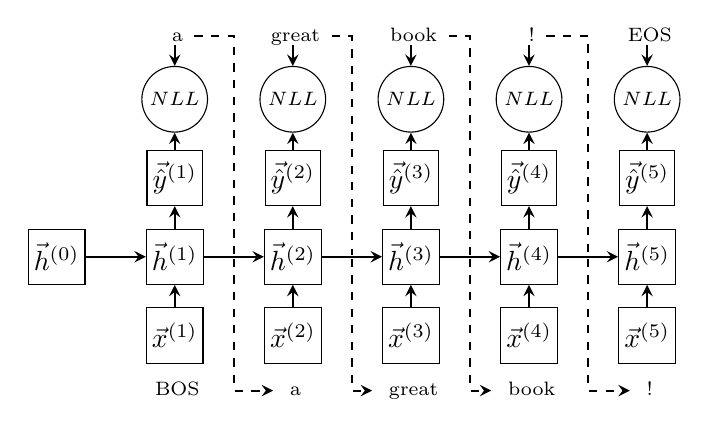
\begin{tikzpicture}
\node (h0) [vec, minimum height=7mm] at (0, 1) {$\vec h^{(0)}$};
\foreach \i/\word in {1/BOS,2/a,3/great,4/book,5/!}{
\node (h\i) [vec, minimum height=7mm] at (\i*1.5, 1) {$\vec h^{(\i)}$};
\node (yhat\i) [vec, minimum height=7mm] at (\i*1.5, 2) {$\vec {\hat{y}}^{(\i)}$};
\node (nll\i) [draw, circle, inner sep=2pt] at (\i*1.5, 3) {\scriptsize $NLL$};
\node (e\i) [vec, minimum height=7mm] at (\i*1.5, 0) {$\vec x^{(\i)}$};
}
\foreach \i/\word in {1/BOS,2/a,3/great,4/book,5/!}{
\node (w\i) [font=\scriptsize, inner sep=0] at (\i*1.5, -.7) {\phantom{A}\word\phantom{g}};
}

\foreach \i/\word in {1/a,2/great,3/book,4/!, 5/EOS}{
\node (y\i) [font=\scriptsize, inner sep=0] at (\i*1.5, 3.8) {\phantom{A}\word\phantom{g}};
}

\foreach \i/\j in {0/1, 1/2, 2/3, 3/4, 4/5}{
\draw [->, >=stealth, thick] (h\i) -- (h\j);
\draw [->, >=stealth, thick] (e\j) -- (h\j);
\draw [->, >=stealth, thick] (h\j) -- (yhat\j);
\draw [->, >=stealth, thick] (yhat\j) -- (nll\j);
\draw [->, >=stealth, thick] (y\j) -- (nll\j);
}
\foreach \i/\j in {1/2, 2/3, 3/4, 4/5}{
\node at ($(h\i)!0.5!(h\j)$) [inner sep=0pt] (p) {};
\draw [->, >=stealth, thick, dashed] (y\i.east)  --(p|-y\i.east) -- (p) -- (p |- w\j.west) -- (w\j.west);
}
\end{tikzpicture}}
\end{center}
\vfill

\end{frame}

\begin{frame}{Self-Attention for AR LM \& Decoding}

\begin{itemize}
\item With attention, all $\vec o_j$ depend on all $\vec v_{j'}$ (and by extension, all $\vec x_{j'}$).
\item This means that the model can easily cheat by looking at future words (red connections)
\end{itemize}
\begin{center}
\resizebox{!}{.55\textheight}{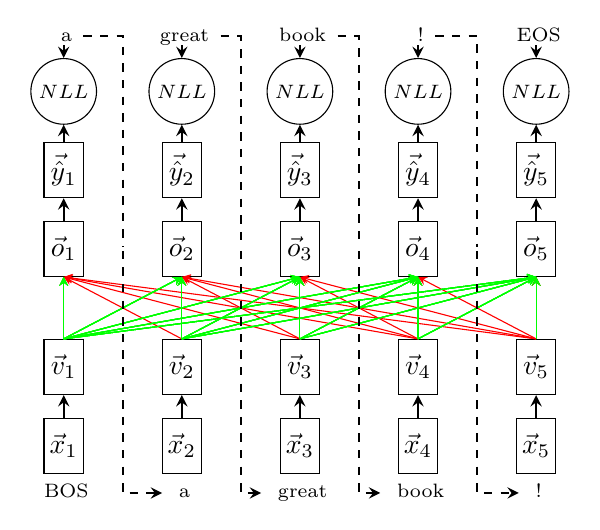
\begin{tikzpicture}
\foreach \i/\word in {1/BOS,2/a,3/great,4/book,5/!}{
\node (h\i) [vec, minimum height=7mm] at (\i*1.5, 1) {$\vec o_\i$};
\node (yhat\i) [vec, minimum height=7mm] at (\i*1.5, 2) {$\vec {\hat{y}}_\i$};
\node (nll\i) [draw, circle, inner sep=2pt] at (\i*1.5, 3) {\scriptsize $NLL$};
\node (e\i) [vec, minimum height=7mm] at (\i*1.5, -.5) {$\vec v_\i$};
\node (x\i) [vec, minimum height=7mm] at (\i*1.5, -1.5) {$\vec x_\i$};
}
\foreach \i/\word in {1/BOS,2/a,3/great,4/book,5/!}{
\node (w\i) [font=\scriptsize, inner sep=0] at (\i*1.5, -2.1) {\phantom{A}\word\phantom{g}};
}

\foreach \i/\word in {1/a,2/great,3/book,4/!, 5/EOS}{
\node (y\i) [font=\scriptsize, inner sep=0] at (\i*1.5, 3.7) {\phantom{A}\word\phantom{g}};
}

\foreach \i/\j in {0/1, 1/2, 2/3, 3/4, 4/5}{
\draw [->, >=stealth, thick] (h\j) -- (yhat\j);
\draw [->, >=stealth, thick] (yhat\j) -- (nll\j);
\draw [->, >=stealth, thick] (y\j) -- (nll\j);
\draw [->, >=stealth, thick] (x\j) -- (e\j);
}
\foreach \i in {1,2,3,4,5}{
\foreach \j in {\i,...,5}{
\draw [<-, >=stealth, red] (h\i.south) -- (e\j.north);
}
\foreach \i in {1,2,3,4,5}{
\foreach \j in {\i,...,5}{
\draw [->, >=stealth, green] (e\i.north) -- (h\j.south);
}
}
}

\foreach \i/\j in {1/2, 2/3, 3/4, 4/5}{
\node at ($(h\i)!0.5!(h\j)$) [inner sep=0pt] (p) {};
\draw [->, >=stealth, thick, dashed] (y\i.east)  --(p|-y\i.east) -- (p) -- (p |- w\j.west) -- (w\j.west);
}
\end{tikzpicture}}
\end{center}

\end{frame}

\begin{vbframe}{Masked Self-Attention}

\vfill

\begin{itemize}
\item So when we use self-attention for language modeling or in a sequence-to-sequence decoder, we have to prevent $\vec o_j$ from attending to any $\vec v_{j'}$ where $j' > j$.
\item \ques How can we do that?
\item Remember:
$$ \begin{aligned}
\vec o_j & = \sum_{j' = 1}^{J} \alpha_{j,j'} \vec v_{j'} \\
 \alpha_{j,j'} & = \frac{\mathrm{exp}(e_{j,j'})}{\sum_{j'' = 1}^J \mathrm{exp}(e_{j,j''})}
\end{aligned}
$$
\begin{itemize}
\item By hardcoding $e_{j,j'} = -\infty$ when $j' > j$ (in practice, ``$\infty$'' is just a large constant)
\item That way, $\mathrm{exp}(e_{j,j'}) = \alpha_{j,j'} = 0$, so $\vec v_{j'}$ has no impact on $\vec o_j$
\end{itemize}
\end{itemize}

\vfill

\end{vbframe}

\begin{vbframe}{Parallelized Masked Self-Attention}

\vfill

\begin{itemize}
\item Step 1: Calculate $\vec E$ like we usually would
\item Step 1B:
$$
\begin{aligned}
\vec E^\mathrm{masked} & = \vec E \odot \vec M + \infty\vec M-\infty; \qquad m_{j,j'} = \begin{cases} 1 & \text{ if } j' \leq j \\ 0 & \text{ otherwise} \end{cases}
\end{aligned}
$$
\item Example:
\end{itemize}
$$
\begin{aligned}
\vec E & = \begin{bmatrix} e_{1,1} & e_{1,2} & e_{1,3} \\ e_{2,1} & e_{2,2} & e_{2,3} \\ e_{3,1} & e_{3,2} & e_{3,3} \end{bmatrix}; \qquad \vec M = \begin{bmatrix} 1 & 0 & 0 \\ 1 & 1 & 0 \\ 1 & 1 & 1 \end{bmatrix} \\
\vec E^\mathrm{masked} & = \begin{bmatrix} e_{1,1} & -\infty & -\infty \\ e_{2,1} & e_{2,2} & -\infty \\ e_{3,1} & e_{3,2} & e_{3,3} \end{bmatrix} ; \qquad \vec A^\mathrm{masked} = \begin{bmatrix} 1 & 0 & 0 \\ \alpha_{2,1} & \alpha_{2,2} & 0 \\ \alpha_{3,1} & \alpha_{3,2} & \alpha_{3,3} \end{bmatrix} \\
\vec o_1 = \vec v_1; \qquad & \vec o_2 = \alpha_{2,1} \vec v_1 + \alpha_{2,2} \vec v_2; \qquad \vec o_3 = \alpha_{3,1} \vec v_1 + \alpha_{3,2} \vec v_2 + \alpha_{3,3} \vec v_3
\end{aligned}
$$

\vfill

\end{vbframe}

\begin{frame}{AR Transformer at Inference Time}

\vfill

\begin{itemize}
\item During training (targets known): Use parallelized masked attention
\item At inference time (targets unknown): Decode prediction in a loop
\item Slower, but at least we don't have to worry about masking anymore
\end{itemize}
\begin{center}
\resizebox{!}{.5\textheight}{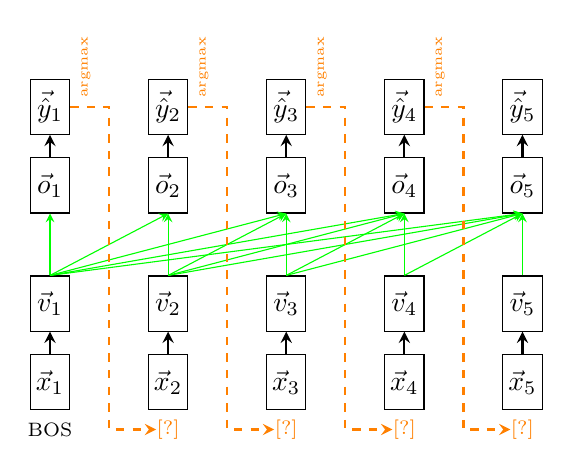
\begin{tikzpicture}
\foreach \i/\word in {1/BOS,2/a,3/great,4/book,5/!}{
\node (h\i) [vec, minimum height=7mm] at (\i*1.5, 1) {$\vec o_\i$};
\node (yhat\i) [vec, minimum height=7mm] at (\i*1.5, 2) {$\vec {\hat{y}}_\i$};
\node (e\i) [vec, minimum height=7mm] at (\i*1.5, -.5) {$\vec v_\i$};
\node (x\i) [vec, minimum height=7mm] at (\i*1.5, -1.5) {$\vec x_\i$};
}
\foreach \i/\word in {2/a,3/great,4/book,5/!}{
\node (w\i) [font=\scriptsize, inner sep=0, orange] at (\i*1.5, -2.1) {[?]};
}
\foreach \i/\word in {1/BOS}{
\node (w\i) [font=\scriptsize, inner sep=0] at (\i*1.5, -2.1) {BOS};
}

\foreach \i/\j in {0/1, 1/2, 2/3, 3/4, 4/5}{
\draw [->, >=stealth, thick] (h\j) -- (yhat\j);
\draw [->, >=stealth, thick] (x\j) -- (e\j);
}
\foreach \i in {1,2,3,4,5}{
\foreach \j in {\i,...,5}{
\draw [->, >=stealth, green] (e\i.north) -- (h\j.south);
}
}

\foreach \i/\j in {1/2, 2/3, 3/4, 4/5}{
\node at ($(h\i)!0.5!(h\j)$) [inner sep=0pt] (p) {};
\draw [->, >=stealth, thick, dashed, orange] (yhat\i.east)  --(p|-yhat\i.east) -- (p) -- (p |- w\j.west) -- (w\j.west);
\node at ([xshift=2mm, yshift=5mm] yhat\i.east) [rotate=90, font=\tiny, orange] {argmax};
}
\end{tikzpicture}}
\end{center}

\vfill

\end{frame}

\begin{vbframe}{Encoder-Decoder Attention}

\vfill

\textbf{\ques How do we connect encoder and decoder?}\\

\vspace{.3cm}

Construction of one decoder block:

\vspace{.3cm}

	\begin{enumerate}
		\item Masked (Multi-Head) Attention layer (only target sequence)
		\item "Ordinary" (Multi-Head) Attention layer
			\begin{itemize}
				\item Queries from the previous decoder layer
				\item Keys, Values from the encoder output
			\end{itemize}
		\item Feed-Forward layer (w/ residual connections \& layer norm)
	\end{enumerate}

\vspace{.3cm}

$\to$ Allows the decoder to attend to \textit{all} tokens from the input sequences\\
(cf. \beamergotobutton{\href{https://arxiv.org/abs/1409.0473}{Bahdanau et al., 2015}} for RNNs)

\vfill

\end{vbframe}

%%%%%%%%%%%%%%%%%%%%%%%%%%%%%%%%%%%%%%%%%%%%%%%%%%%%%%%%%%%%%%%%%%

\section{Transformer Parameter Count}
%%%%%%%%%%%%%%%%%%%%%%%%%%%%%%%%%%%%%%%%%%%%%%%%%%%%%%%%%%%%%%%%%%

\begin{frame}{Overview over Parameter Sources}
\vfill
\begin{minipage}[c]{.49\textwidth}
    \vfill
    \begin{figure}
		\centering
		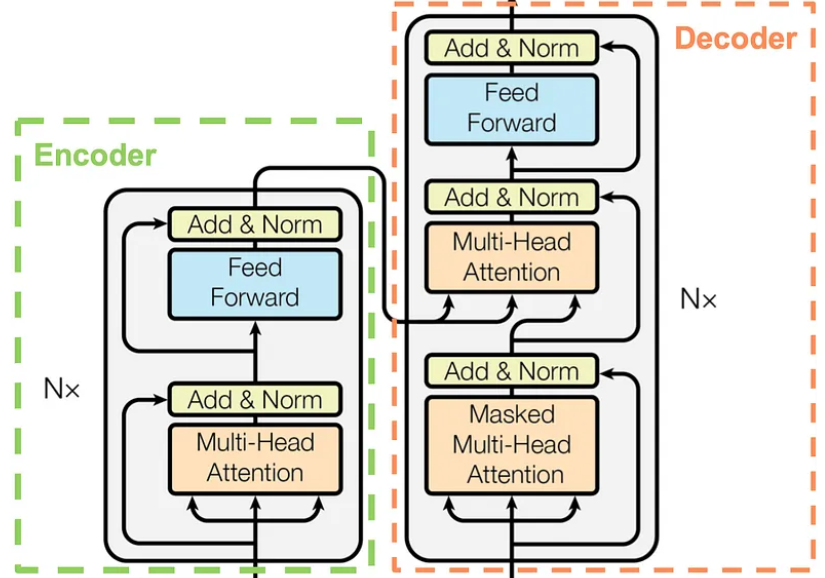
\includegraphics[]{figure/enc_dec.png}
	\end{figure}
    \vfill
\end{minipage}
\hfill
\begin{minipage}[c]{.49\textwidth}
    \hfill
    \begin{itemize}
        \item \textbf{Encoder}
        \begin{itemize}
            \item Multi-Head Attention
            \item 2x Layernorm
            \item Feed Forward Network
        \end{itemize}
        \item \textbf{Decoder}
        \begin{itemize}
            \item 2x Multi-Head Attention
            \item 3x Layernorm
            \item Feed Forward Network
        \end{itemize}
        \item \textbf{Original sizes:} $d_{model} = 512$, $n_{head} = 8$, so $d_{qkv} = 512/8 = 64$
    \end{itemize}
\end{minipage}
\vfill
\textit{Derive the parameter count of each component, then sum them up!} \citebutton{Vaswani et al., 2017}{https://arxiv.org/abs/1706.03762}

\end{frame}

\begin{frame}{Multi-Head Attention}

\begin{minipage}[c]{.34\textwidth}
    \begin{figure}
        \centering
        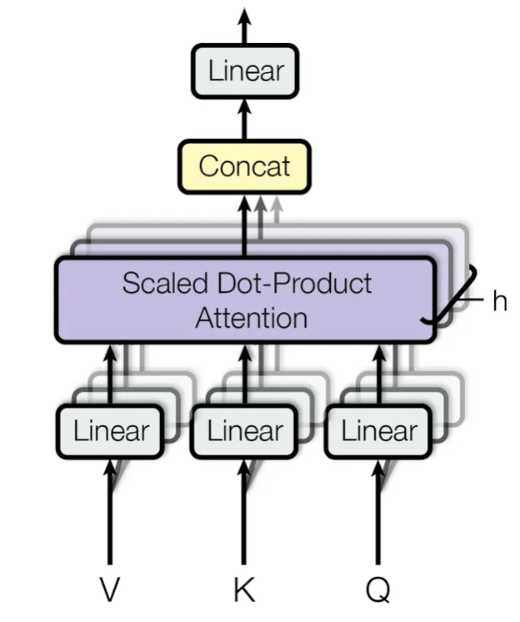
\includegraphics[width=\linewidth]{figure/mha.png}
    \end{figure}
\end{minipage}
\hfill
\begin{minipage}[c]{.63\textwidth}
    \begin{itemize}
        \item Per head: $\boldsymbol{W_Q}, \boldsymbol{W_K}, \boldsymbol{W_V}$, each $d_{model} \times d_{qkv}$ (plus bias), with $d_{qkv} = d_{model}/n_{head}$
        \item Concatenating the $n_{head}$ outputs gives $d_{model}$ again; $\boldsymbol{W_O}$ is $d_{model} \times d_{model}$ (plus bias)
    \end{itemize}
\end{minipage}

$$
\begin{aligned}
N_{attention} &= \underbrace{(d_{model}^2 + d_{model})}_{W_O} + \underbrace{(d_{model} \cdot d_{qkv} + d_{qkv}) \cdot n_{head} \cdot 3}_{W_{Q,K,V}\text{ of all heads}} \\
&= (d_{model}^2 + d_{model}) \cdot 4 \;\approx\; 4 \cdot d_{model}^2
\end{aligned}
$$

\end{frame}

\begin{frame}{Feed-Forward Network and Layer Norm}

\begin{minipage}[c]{.3\textwidth}
    \centering
    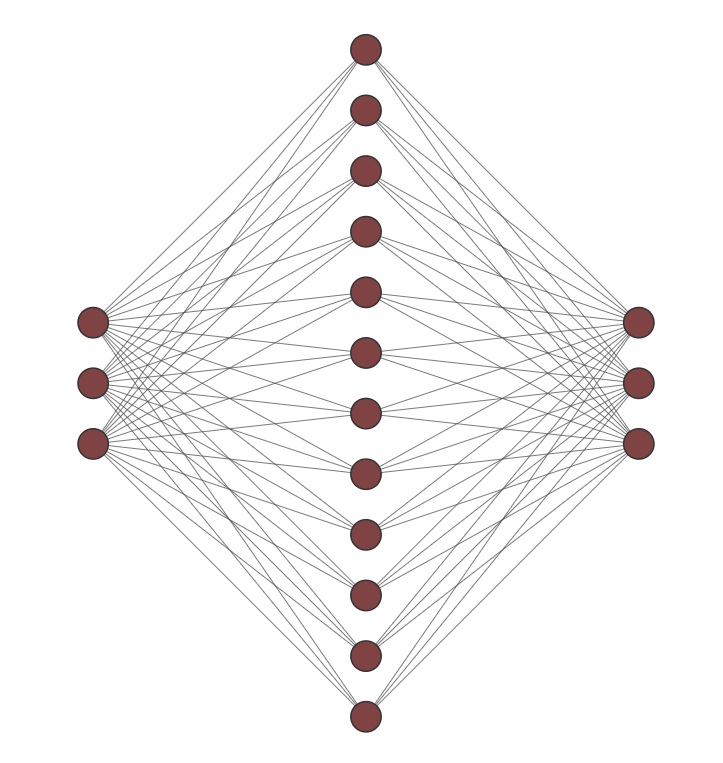
\includegraphics[width=\linewidth,height=3.2cm,keepaspectratio]{figure/ffn.png}
\end{minipage}
\hfill
\begin{minipage}[c]{.66\textwidth}
    \begin{itemize}
        \item The FFN of the Transformer uses two fully connected layers, $d_{model} \to 4\cdot d_{model} \to d_{model}$ (the factor 4 is a design decision by the authors of the paper)
        \item Weight matrices $W_1$: $d_{model} \times 4\cdot d_{model}$ and $W_2$: $4\cdot d_{model} \times d_{model}$, plus biases
    \end{itemize}
\end{minipage}

\begin{align*}
N_{FFN} &= (4 d_{model}^2 + 4 d_{model}) + (4 d_{model}^2 + d_{model}) \\
&= 8 d_{model}^2 + 5 d_{model} \approx 8 d_{model}^2
\end{align*}

\textbf{Layer norm:} one $\gamma$ and one $\beta$ per dimension (see the Layer Normalization frame), so $N_{Layernorm} = 2\cdot d_{model}$.

\end{frame}

\begin{frame}{Total Parameter Count}

{\small
\begin{align*}
N_{Encoder} &= N_{attention} + N_{FFN} + 2\cdot N_{Layernorm} = 12\, d_{model}^2 + 13\, d_{model} \\
N_{Decoder} &= 2\cdot N_{attention} + N_{FFN} + 3\cdot N_{Layernorm} = 16\, d_{model}^2 + 19\, d_{model}
\end{align*}}

\begin{itemize}
    \item Vanilla Transformer: $n_{Layers} = 6$ for both Encoder and Decoder, $d_{model} = 512$
    \item Exact: $\;6\cdot(12\cdot 512^2 + 13\cdot 512) + 6\cdot(16\cdot 512^2 + 19\cdot 512) = 44,138,496$
    \item Approximate: $\;6\cdot(12\cdot 512^2) + 6\cdot(16\cdot 512^2) = 44,040,192$
\end{itemize}

\textit{The count scales quadratically with $d_{model}$, so bias and layer norm terms are negligible --- $28\cdot d_{model}^2$ per encoder+decoder layer pair is a good approximation.}

\end{frame}

\begin{frame}{Embedding Parameters}

\textit{We also have to consider the parameters of the embeddings!}

\begin{itemize}
    \item Let $M$ be the maximum sequence length and $V$ the size of the vocabulary
    \item We have $M \times d_{model}$ positional embedding parameters, which are fixed and not learned
    \item And $V \times d_{model}$ token embedding parameters, which are learned
    \item The original transformer has $V = 37000$ tokens:
			$$N_{Embedding} = 37000 \cdot 512 = 18,944,000$$
		\item Adding those to the previous count yields:
			$$N_{Final} = 18,944,000 + 44,040,192 = 62,984,192$$

\end{itemize}

\end{frame}

%%%%%%%%%%%%%%%%%%%%%%%%%%%%%%%%%%%%%%%%%%%%%%%%%%%%%%%%%%%%%%%%%%

\section{Efficient Transformers}
%%%%%%%%%%%%%%%%%%%%%%%%%%%%%%%%%%%%%%%%%%%%%%%%%%%%%%%%%%%%%%%%%%

\begin{frame}{Limitation of the Transformer}
\small

\vfill

\begin{figure}
\centering
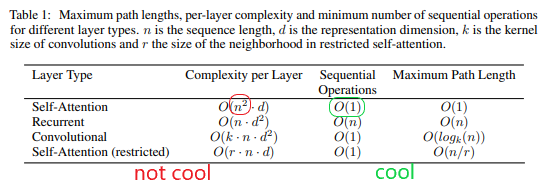
\includegraphics[width = 5.5cm]{figure/n_squared.png}\\
\footnotesize{Source:} \href{https://arxiv.org/pdf/1706.03762.pdf}{\footnotesize Vaswani et al. (2017)}
\end{figure}

\textbf{Advantage:}

\begin{itemize}
	\item Every token can \textit{directly} attend to each other token
	\item Cf. RNN: At worst $n$ sequential operations (last to first token)
\end{itemize}

\textbf{Severe Limitation:}

\begin{itemize}
	\item Every token attends to each other token (incl. itself)\\
				$\to$ We need to calculate $n^2$ attention weights
	\item Computational complexity of Transformer scales quadratically with the sequence length\\
				$\to$ Longer sequences are disproportionally expensive
\end{itemize}

\vfill

\end{frame}

\begin{frame}{Efficient Transformers}

\footnotesize
\textbf{Broad overview on so-called "X-formers"} \beamergotobutton{\href{https://arxiv.org/pdf/2009.06732.pdf}{Tay et al., 2020a}}

\begin{itemize}
	\item Efficient \& fast Transformer-based models\\
				$\rightarrow$ Reduce complexity from $\mathcal{O}(n^2)$ to (up to) $\mathcal{O}(n)$
	\item Claim on-par (or even) superior performance
	\item Different techniques used:
				\begin{itemize}
					\item Fixed/Factorized/Random Patterns
					\item Learnable Patterns (extension of the above)
					\item Low-Rank approximations or Kernels
					\item Recurrence (see e.g. \beamergotobutton{\href{https://arxiv.org/pdf/1901.02860.pdf}{Dai et al., 2019}})
					\item Memory modules
				\end{itemize}
\end{itemize}

	\vspace{.3cm}

\textbf{Side note:}

\begin{itemize}
	\item Most benchmark data sets not explicitly designed for evaluating long-range abilities of the models.
	\item Recently proposed: \textit{Long Range Arena: A benchmark for efficient transformers} \beamergotobutton{\href{https://arxiv.org/pdf/2011.04006.pdf}{Tay et al., 2020b}}
\end{itemize}

\vfill

\end{frame}

\begin{frame}{Efficient Transformers}

\vfill

	\begin{figure}
		\centering
		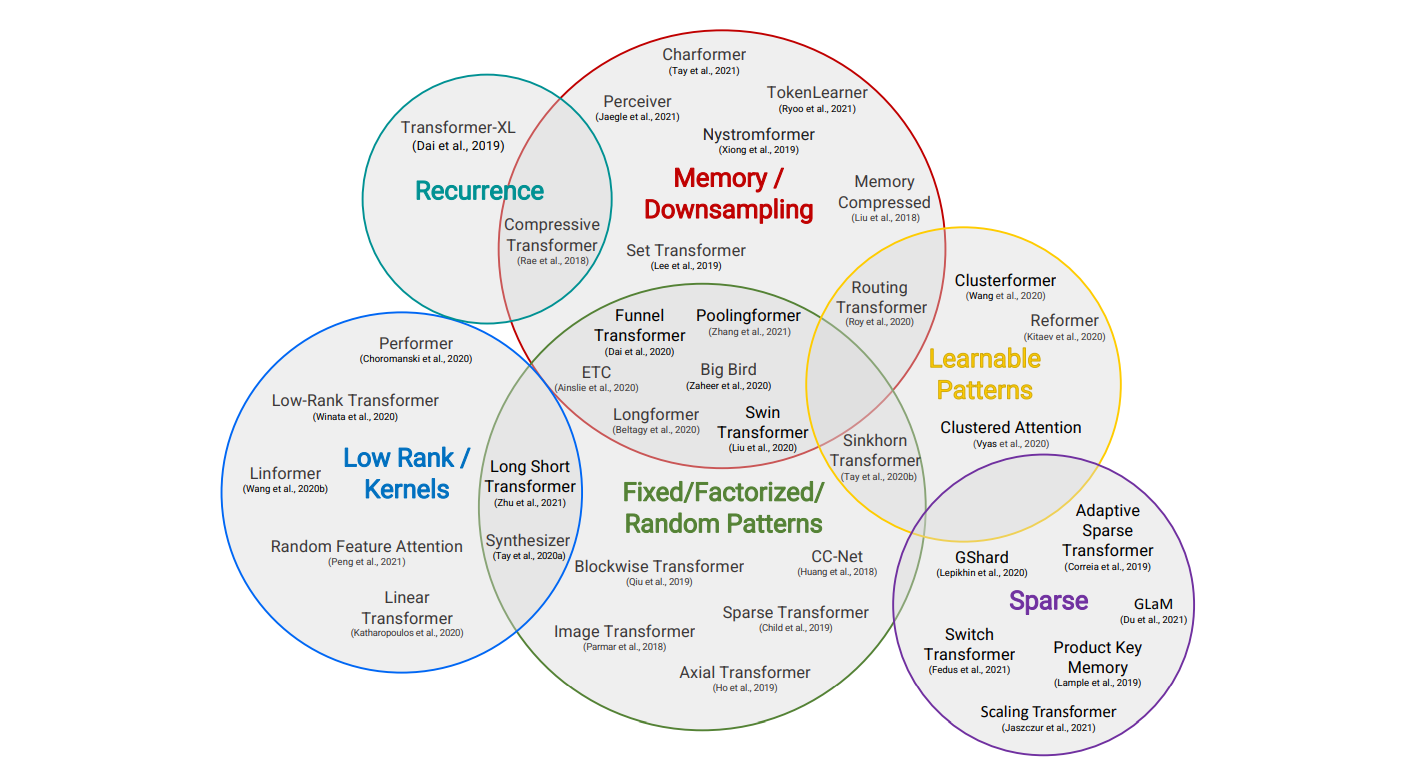
\includegraphics[width = 11cm]{figure/tay-xformers.png}\\
		\beamergotobutton{\href{https://arxiv.org/pdf/2009.06732.pdf}{Tay et al., 2020a}}
	\end{figure}

\vfill

\end{frame}

\begin{frame}{Sparse Attention: Fixed Patterns}
\footnotesize
Idea: most query-key pairs contribute little, so compute only a fixed, sparse subset of the attention matrix (white cells = skipped). \beamergotobutton{\href{https://proceedings.neurips.cc//paper/2020/file/c8512d142a2d849725f31a9a7a361ab9-Paper.pdf}{Source: Zaheer et al., 2020}}
\begin{center}
	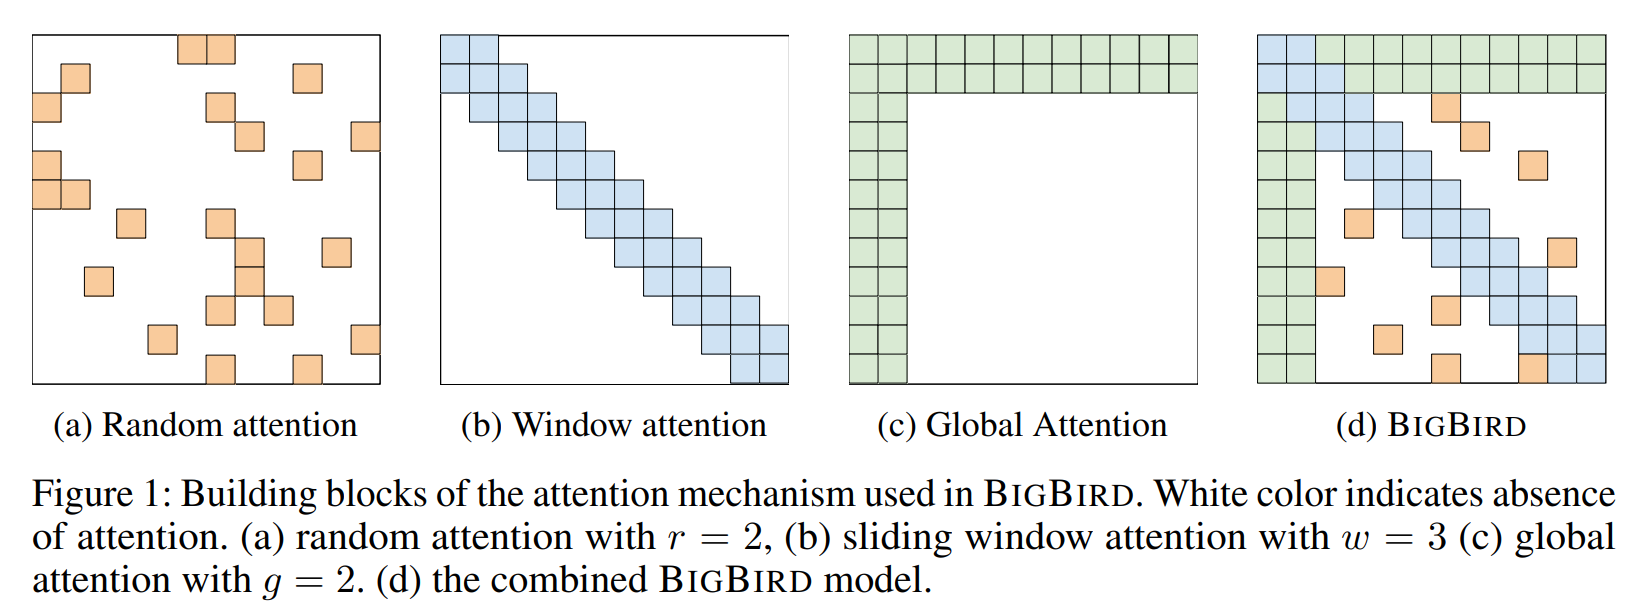
\includegraphics[width = 7.5cm]{figure/bigbird-patterns.png}
\end{center}
\vspace{-2mm}
\begin{itemize}
	\item \textbf{(a) Random}: each query attends to a few randomly chosen keys
	\item \textbf{(b) Window (local)}: each query attends only to its neighbours, $|i-j| \le w$ --- the decoder's causal mask is the one-sided version of the same idea
	\item \textbf{(c) Global}: a few tokens attend to, and are attended by, every position --- one cheap channel for long-range information
	\item \textbf{(d) BigBird} combines all three; Longformer (Beltagy et al., 2020) uses (b) + (c)
\end{itemize}
\end{frame}

\begin{frame}{Efficient Transformers --- Tradeoff}

\vfill

\begin{itemize}
	\item \textit{Quality:} How well can we approximate the results we would get when applying full attention?
	\item[]
	\item \textit{Speed:} Can we reduce the computational complexity from quadratic to (nearly) linear?
\end{itemize}

\vfill

\end{frame}

\begin{frame}{A Primer on Flash Attention}

\vfill

\textbf{Compute-bound vs. memory-bound operations:}

\begin{itemize}
	\item Wall-clock time not (necessarily) a function of FLOPs
	\item Most of these ``Efficient Transformers`` focus on FLOP reduction
	\item[] $\to$ This ignores existing memory overheads
	\item \textit{Compute-bound operations:} ($\approx$ FLOPs)
			\begin{itemize}
				\item Matrix multiplication
			\end{itemize}
	\item \textit{Memory-bound operations:} ($\approx$ data transfer)
			\begin{itemize}
				\item Attention
			\end{itemize}
\end{itemize}

\vfill

\end{frame}

\begin{frame}{A Primer on Flash Attention}

\vfill

	\begin{figure}
		\centering
		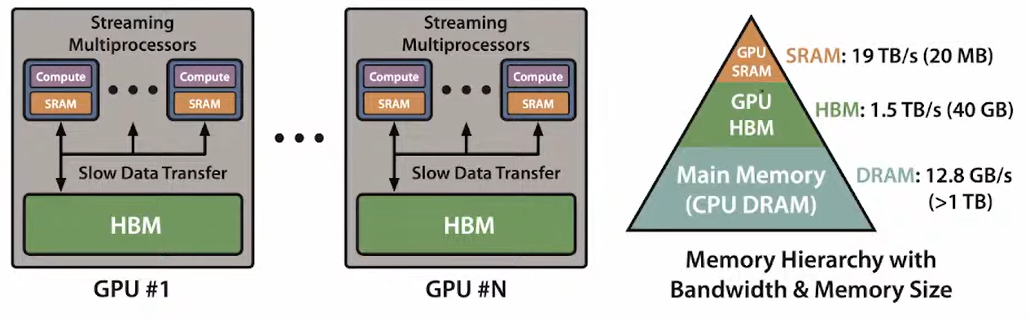
\includegraphics[width = 11cm]{figure/memory-hierarchy2.png}\\
		\beamergotobutton{\href{https://www.youtube.com/watch?v=gMOAud7hZg4}{Source: Talk by Tri Dao, 2023}}
	\end{figure}

\vfill

\end{frame}

\begin{frame}{A Primer on Flash Attention}

\begin{minipage}[c]{.49\textwidth}
\vfill
	\begin{figure}
		\centering
		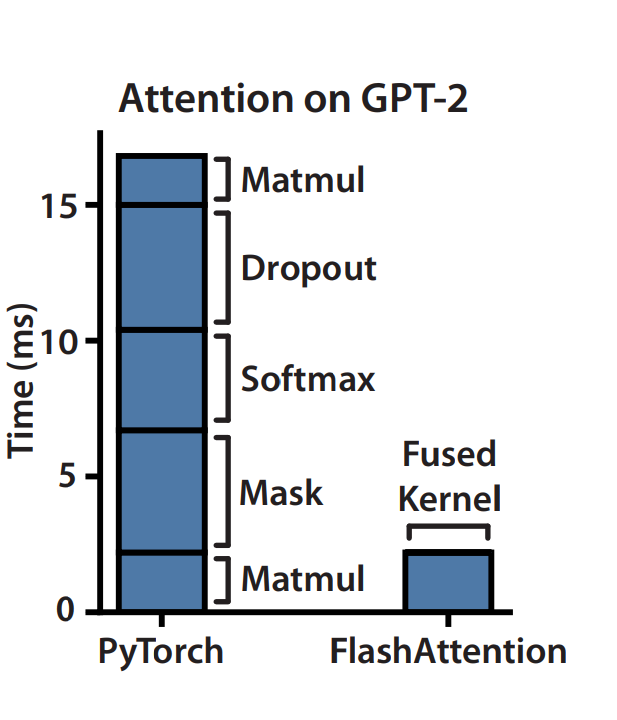
\includegraphics[width = 5cm]{figure/flash-attn.png}\\
		\beamergotobutton{\href{https://arxiv.org/abs/2205.14135}{Source: Dao, 2022}}
	\end{figure}
	\vfill
\end{minipage}
\hfill
\begin{minipage}[c]{.49\textwidth}
	\begin{itemize}
	\item \textit{Compute-bound operations:}
			\begin{itemize}
				\item Matmul
			\end{itemize}
	\item \textit{Memory-bound operations:}
			\begin{itemize}
				\item Mask
				\item Dropout
				\item Softmax
			\end{itemize}
	\item[] $\to$ Reducing memory-bound operations most effective for reducing wall-clock time
	\end{itemize}
\end{minipage}

\end{frame}

%%%%%%%%%%%%%%%%%%%%%%%%%%%%%%%%%%%%%%%%%%%%%%%%%%%%%%%%%%%%%%%%%%

\section{Long Sequences: Transformer-XL}
%%%%%%%%%%%%%%%%%%%%%%%%%%%%%%%%%%%%%%%%%%%%%%%%%%%%%%%%%%%%%%%%%%

\begin{frame}{Transformer-XL}
\small

\vfill

\textbf{Key facts:}

\begin{itemize}
	\item Objective: Autoregressive Language Modeling task
	\item Transformer decoder model
	\item Addresses long sequences
	\item Assumption: \textit{No} infinite memory \& compute; limited resources
	\item (Possible) Solution Vanilla Transformer:
		\begin{itemize}
			\item Split corpus into shorter segments
			\item Limited contextual information
		\end{itemize}
	\item Solution Transformer-XL:
		\begin{itemize}
			\item Segment-level recurrence mechanism
			\item Able to model longer-term dependencies
		\end{itemize}
\end{itemize}

\vfill

\end{frame}

\begin{frame}{Transformer-XL}

\begin{figure}
\centering
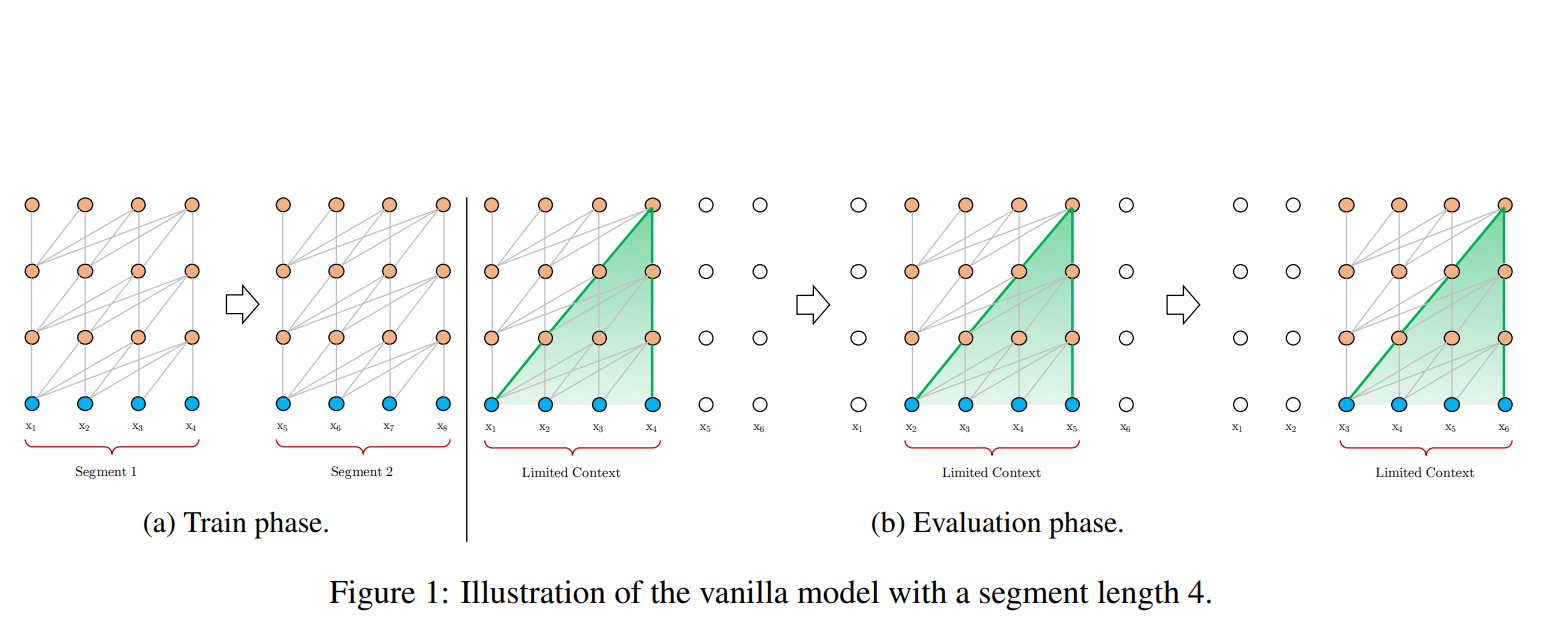
\includegraphics[width = 10.5cm]{figure/vanilla-trafo-seq4.png}\\
\footnotesize{Source:} \href{https://aclanthology.org/P19-1285.pdf}{\footnotesize Dai et al. (2019)}
\end{figure}

\begin{itemize}
		\item Contextual information limited to segments
		\item Does not respect semantic or syntactic boundaries
\end{itemize}

\end{frame}

\begin{vbframe}{Transformer-XL}

\begin{figure}
\centering
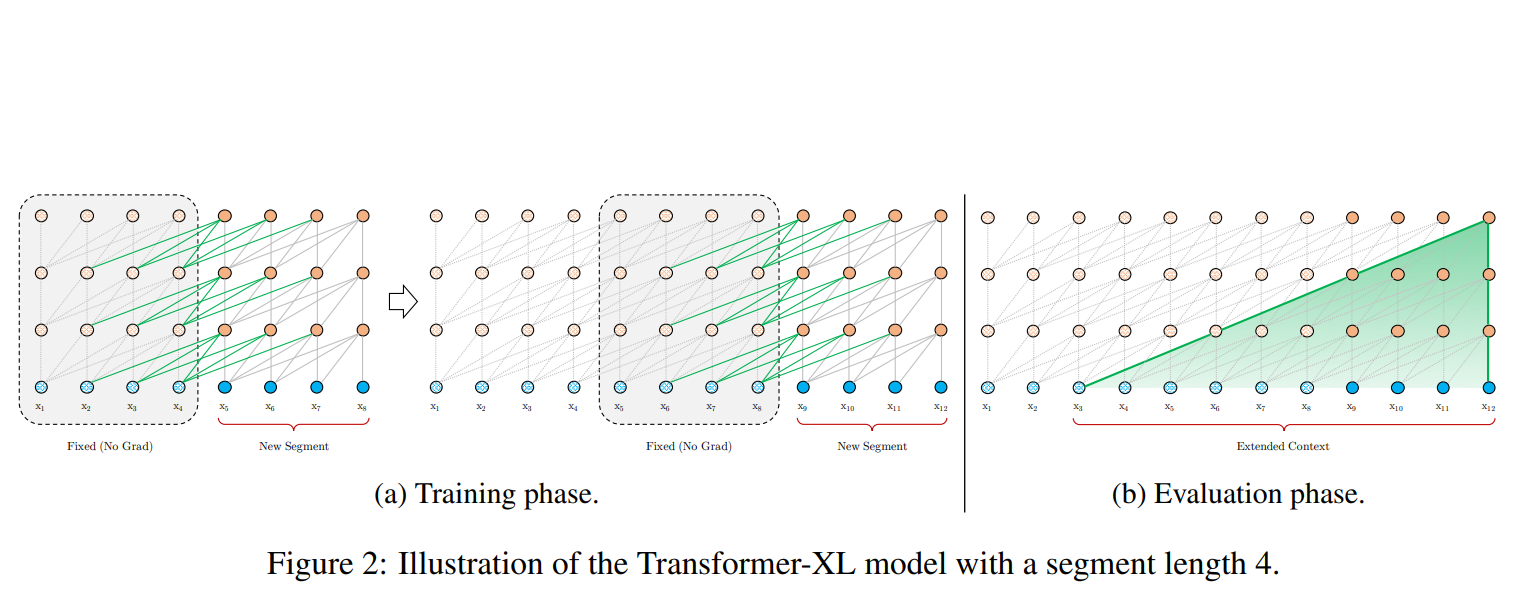
\includegraphics[width = 11.5cm]{figure/trafo-xl-seq4.png}\\
\footnotesize{Source:} \href{https://aclanthology.org/P19-1285.pdf}{\footnotesize Dai et al. (2019)}
\end{figure}

\begin{itemize}
		\item Caches hidden states from the previous segment
		\item Contextual information flows across segments
\end{itemize}

\end{vbframe}

\begin{vbframe}{Segment Recurrence}

\begin{itemize}
		\item Let $s_\tau = [x_{\tau,1}, \hdots, x_{\tau,L}]$ and $s_{\tau+1} = [x_{\tau+1,1}, \hdots, x_{\tau+1,L}]$ be two consecutive segments of length $L$.
		\item Let $h_\tau^n \in \mathds{R}^{L\times d}$ denote the $n$-th layer hidden states for $s_\tau$.
		\item Using segment recurrence, the $n$-th layer hidden states for the following segment $s_{\tau+1}$ are computed as follows:
\end{itemize}

$$\tilde{h}_{\tau+1}^{n-1} = Concat[SG(h_{\tau}^{n-1}), h_{\tau+1}^{n-1}]$$

$$q_{\tau+1}^{n} = h_{\tau+1}^{n-1}W^\text{T}_q; \quad k_{\tau+1}^{n} = \tilde{h}_{\tau+1}^{n-1}W^\text{T}_k; \quad v_{\tau+1}^{n} = \tilde{h}_{\tau+1}^{n-1}W^\text{T}_v$$

$$h_{\tau+1}^{n} = Trafo(q_{\tau+1}^{n}, k_{\tau+1}^{n}, v_{\tau+1}^{n}),$$

\begin{itemize}
		\item[] where $SG(\cdot)$ stands for "`stop-gradient"'.
\end{itemize}

\end{vbframe}

\begin{vbframe}{Relative Positional Encodings}

\vfill

\textbf{Problem:}

\begin{itemize}
	\item \textit{Absolute} positional encodings (PE) would assign the same embedding to words in similar positions in both segments
	\item No positional difference between $x_{\tau,j}$ and $x_{\tau+1,j}$
\end{itemize}

\textbf{Solution:}

\begin{itemize}
	\item Inject information about the relative distance between a query vector and the respective key vectors directly into the Attention mechanism
	\item \textit{Comment:} Using relative PEs utterly necessary here, but also applicable independently of the segment recurrence
\end{itemize}

\begin{align*}
	\rmA_{i,j}^\text{abs}
	&= \underbrace{ \rmE_{x_i}^\top \rmW_q^\top \rmW_k \rmE_{x_j} }_{(a)}
	+ \underbrace{\rmE_{x_i}^\top \rmW_q^\top \rmW_k \rmU_{j}}_{(b)} \\
	&+ \underbrace{\rmU_{i}^\top \rmW_q^\top \rmW_k \rmE_{x_j}}_{(c)}
	+ \underbrace{\rmU_{i}^\top \rmW_q^\top \rmW_k \rmU_{j}}_{(d)}. \vspace{-0.5em}
\end{align*}

\begin{align*}
	\rmA_{i,j}^\text{rel}
	&= \underbrace{ \rmE_{x_i}^\top \rmW_q^\top \rmW_{k,E} \rmE_{x_j} }_{(a)}
	+ \underbrace{\rmE_{x_i}^\top \rmW_q^\top \rmW_{k,R} \rmR_{i-j} }_{(b)} \\
	&+ \underbrace{u^\top \rmW_{k,E} \rmE_{x_j}}_{(c)}
	+ \underbrace{v^\top \rmW_{k,R} \rmR_{i-j}}_{(d)}.
\end{align*}

\end{vbframe}

\begin{vbframe}{Relative Positional Encodings}

\vfill

\textbf{Solution:}

\begin{itemize}
	\item Replace all absolute PEs with relative ones (fixed $+$ sinusoidal)\\
				$\to$ $\rmR_{i-j}$ instead of $\rmU_{j}$ in (b) and (d)
	\item Replace all positional query vectors with single trainable embeddings\\
				$\to$ $u$ and $v$ instead of $\rmU_{i}^\top \rmW_q^\top$ in (c) and (d)
	\item Use separate weight matrices for linearly projecting $\rmE$\\
				$\to$ $\rmW_{k,E}$ and $\rmW_{k,R}$ instead of $\rmW_{k}$
\end{itemize}

\vfill

\end{vbframe}

%%%%%%%%%%%%%%%%%%%%%%%%%%%%%%%%%%%%%%%%%%%%%%%%%%%%%%%%%%%%%%%%%%

\section{The Three Transformer Families}
%%%%%%%%%%%%%%%%%%%%%%%%%%%%%%%%%%%%%%%%%%%%%%%%%%%%%%%%%%%%%%%%%%

\begin{vbframe}{Encoder-Only, Decoder-Only, Encoder-Decoder}
\begin{itemize}
  \item You have now seen both halves of the original Transformer. In practice, most models use only one half, or both, depending on the task:
\end{itemize}
\begin{center}
\footnotesize
\begin{tabular}{@{}p{2.1cm}p{2.8cm}p{2.6cm}p{3.2cm}@{}}
\toprule
 & \textbf{Encoder-only} & \textbf{Decoder-only} & \textbf{Encoder-decoder} \\
\midrule
Attention & bidirectional & causal (masked) & both (+ cross-attn.) \\[2pt]
Pretraining obj. & masked LM & next-token & varies (e.g.\ span corruption) \\[2pt]
Typical use & understanding, embedding & generation & sequence-to-sequence \\[2pt]
Flagship model & BERT & GPT & original Transformer, T5 \\
\bottomrule
\end{tabular}
\end{center}
\begin{itemize}
  \item \textbf{Encoder-only} (bidirectional self-attention, no causal mask): good at building rich representations of an already-complete input --- classification, embeddings, retrieval.
  \item \textbf{Decoder-only} (causal self-attention only): good at generating one token at a time --- today's LLMs are almost all decoder-only.
  \item \textbf{Encoder-decoder} (bidirectional encoder + causal decoder + cross-attention): good at mapping one sequence to another --- translation, summarization.
\end{itemize}
\end{vbframe}

\begin{vbframe}{Where This Is Going}
\begin{itemize}
  \item Session 8 trains all three families into pretrained models --- GPT (decoder-only), BERT (encoder-only), T5 (encoder-decoder) --- and shows how they are used: decoding, prompting, instruction tuning.
  \item Session 10 shows this taxonomy is not NLP-specific: the same patterns reappear in vision and multimodal models.
  \item Nothing about encoder-only, decoder-only, or encoder-decoder is specific to text: what actually distinguishes the three families is which positions are allowed to attend to which other positions, not the domain of the input.
\end{itemize}
\end{vbframe}

%%%%%%%%%%%%%%%%%%%%%%%%%%%%%%%%%%%%%%%%%%%%%%%%%%%%%%%%%%%%%%%%%%
%%%%%%%%%%%%%%%%%%          REFERENCES          %%%%%%%%%%%%%%%%%%
%%%%%%%%%%%%%%%%%%%%%%%%%%%%%%%%%%%%%%%%%%%%%%%%%%%%%%%%%%%%%%%%%%
\begin{vbframe}
\frametitle{References}
\footnotesize{
\begin{thebibliography}{99}
\bibitem[(Bahdanau et al., 2015)]{trans1} Bahdanau, D., Cho, K., \& Bengio, Y. (2015). \textit{Neural Machine Translation by Jointly Learning to Align and Translate}. Published as a conference paper at ICLR 2015. \url{https://arxiv.org/abs/1409.0473}
\bibitem[(Vaswani et al., 2017)]{trans2} Vaswani, A., Shazeer, N., Parmar, N., Uszkoreit, J., Jones, L., Gomez, A. N., Kaiser, {\L}., \& Polosukhin, I. (2017). \textit{Attention Is All You Need}. \url{https://arxiv.org/abs/1706.03762}
\bibitem[(Graves et al., 2014)]{trans5} Graves, A., Wayne, G., \& Danihelka, I. (2014). \textit{Neural Turing Machines}. \url{https://arxiv.org/abs/1410.5401}
\bibitem[(Wang et al., 2019)]{trans6} Wang, Q., Li, B., Xiao, T., Zhu, J., Li, C., Wong, D. F., \& Chao, L. S. (2019). \textit{Learning Deep Transformer Models for Machine Translation}. ACL 2019. \url{https://aclanthology.org/P19-1176/}
\bibitem[(Beltagy et al., 2020)]{trans7} Beltagy, I., Peters, M. E., \& Cohan, A. (2020). \textit{Longformer: The Long-Document Transformer}. \url{https://arxiv.org/abs/2004.05150}
\bibitem[(Fleuret, 2023)]{trans12} Fleuret, F. (2023). \textit{Deep Learning} (course notes), University of Geneva. \url{https://fleuret.org/dlc/}, \S13.1--13.3. Licensed CC BY-NC-SA 4.0.
\end{thebibliography}
}
\end{vbframe}


%%%%%%%%%%%%%%%%%%%%%%%%%%%%%%%%%%%%%%%%%%%%%%%%%%%%%%%%%%%%%%%%%%

\section{License \& Attribution}
%%%%%%%%%%%%%%%%%%%%%%%%%%%%%%%%%%%%%%%%%%%%%%%%%%%%%%%%%%%%%%%%%%

\begin{vbframe}{License \& Attribution}
\begin{itemize}
\item \textbf{Main source.} All sections except those listed below are adapted from \textbf{Deep Learning for NLP (DL4NLP)}, SLDS, LMU Munich --- licensed \textbf{CC BY 4.0}: \url{https://creativecommons.org/licenses/by/4.0/}. Chapter 3 (\textit{Transformer}) is the backbone; chapter 2 provides Root 2 (encoder-decoder RNNs, Bahdanau attention), the basic attention recipe, and tokenization. Frames were reordered, some merged or condensed (word-order proof, parameter count, tokenization), and a few retitled.
\item \textbf{Fleuret.} The Neural Turing Machine root (Root 1), the permutation-invariance frame, and the pre-norm/post-norm frame are freshly drafted following the framing and citations of \textbf{François Fleuret's \textit{Deep Learning} course}, University of Geneva (\url{https://fleuret.org/dlc/}, \S13.1--13.3) --- licensed \textbf{CC BY-NC-SA 4.0}: non-commercial academic teaching use is permitted, reuse must be attributed and shared under the same license.
\item \textbf{Original to this course.} The opening \enquote{Why Attention?} and \enquote{Position-Fixed vs.\ Content-Based Weighting} frames, the explanatory text of the Bahdanau frames, the sparse-attention patterns frame (figure from DL4NLP), and \enquote{The Three Transformer Families} section.
\end{itemize}
\end{vbframe}

\endlecture
\end{document}

